% ******************************* PhD Thesis Template **************************
% Please have a look at the README.md file for info on how to use the template

\documentclass[a4paper,12pt,times,numbered,print,index]{Classes/PhDThesisPSnPDF}

% ******************************************************************************
% ******************************* Class Options ********************************
% *********************** See README for more details **************************
% ******************************************************************************

% `a4paper'(The University of Cambridge PhD thesis guidelines recommends a page
% size a4 - default option) or `a5paper': A5 Paper size is also allowed as per
% the Cambridge University Engineering Deparment guidelines for PhD thesis
%
% `11pt' or `12pt'(default): Font Size 10pt is NOT recommended by the University
% guidelines
%
% `oneside' or `twoside'(default): Printing double side (twoside) or single
% side.
%
% `print': Use `print' for print version with appropriate margins and page
% layout. Leaving the options field blank will activate Online version.
%
% `index': For index at the end of the thesis
%
% `draftclassic': For draft mode without loading any images (same as draft in book)
%
% `draft': Special draft mode with line numbers, images, and water mark with
% timestamp and custom text. Position of the text can also be modified.
%
% `abstract': To generate only the title page and abstract page with
% dissertation title and name, to submit to the Student Registry
%
% `chapter`: This option enables only the specified chapter and it's references
%  Useful for review and corrections.
%
% ************************* Custom Page Margins ********************************
%
% `custommargin`: Use `custommargin' in options to activate custom page margins,
% which can be defined in the preamble.tex. Custom margin will override
% print/online margin setup.
%
% *********************** Choosing the Fonts in Class Options ******************
%
% `times' : Times font with math support. (The Cambridge University guidelines
% recommend using times)
%
% `fourier': Utopia Font with Fourier Math font (Font has to be installed)
%            It's a free font.
%
% `customfont': Use `customfont' option in the document class and load the
% package in the preamble.tex
%
% default or leave empty: `Latin Modern' font will be loaded.
%
% ********************** Choosing the Bibliography style ***********************
%
% `authoryear': For author-year citation eg., Krishna (2013)
%
% `numbered': (Default Option) For numbered and sorted citation e.g., [1,5,2]
%
% `custombib': Define your own bibliography style in the `preamble.tex' file.
%              `\RequirePackage[square, sort, numbers, authoryear]{natbib}'.
%              This can be also used to load biblatex instead of natbib
%              (See Preamble)
%
% **************************** Choosing the Page Style *************************
%
% `default (leave empty)': For Page Numbers in Header (Left Even, Right Odd) and
% Chapter Name in Header (Right Even) and Section Name (Left Odd). Blank Footer.
%
% `PageStyleI': Chapter Name next & Page Number on Even Side (Left Even).
% Section Name & Page Number in Header on Odd Side (Right Odd). Footer is empty.
%
% `PageStyleII': Chapter Name on Even Side (Left Even) in Header. Section Number
% and Section Name in Header on Odd Side (Right Odd). Page numbering in footer

% Uncomment to change page style
%\pagestyle{PageStyleII}


% ********************************** Preamble **********************************
% Preamble: Contains packages and user-defined commands and settings
% ******************************************************************************
% ****************************** Custom Margin *********************************

% Add `custommargin' in the document class options to use this section
% Set {innerside margin / outerside margin / topmargin / bottom margin}  and
% other page dimensions
\ifsetCustomMargin
  \RequirePackage[left=37mm,right=30mm,top=30mm,bottom=30mm]{geometry}
  \setFancyHdr % To apply fancy header after geometry package is loaded
\fi

% Add spaces between paragraphs
%\setlength{\parskip}{0.5em}
% Ragged bottom avoids extra whitespaces between paragraphs
\raggedbottom
% To remove the excess top spacing for enumeration, list and description
%\usepackage{enumitem}
%\setlist[enumerate,itemize,description]{topsep=0em}

% *****************************************************************************
% ******************* Fonts (like different typewriter fonts etc.)*************

% Add `customfont' in the document class option to use this section

\ifsetCustomFont
  % Set your custom font here and use `customfont' in options. Leave empty to
  % load computer modern font (default LaTeX font).
  %\RequirePackage{helvet}

  % For use with XeLaTeX
  %  \setmainfont[
  %    Path              = ./libertine/opentype/,
  %    Extension         = .otf,
  %    UprightFont = LinLibertine_R,
  %    BoldFont = LinLibertine_RZ, % Linux Libertine O Regular Semibold
  %    ItalicFont = LinLibertine_RI,
  %    BoldItalicFont = LinLibertine_RZI, % Linux Libertine O Regular Semibold Italic
  %  ]
  %  {libertine}
  %  % load font from system font
  %  \newfontfamily\libertinesystemfont{Linux Libertine O}
\fi

% *****************************************************************************
% **************************** Custom Packages ********************************

% ************************* Algorithms and Pseudocode **************************

%\usepackage{algpseudocode}


% ********************Captions and Hyperreferencing / URL **********************

% Captions: This makes captions of figures use a boldfaced small font.
%\RequirePackage[small,bf]{caption}

\RequirePackage[labelsep=space,tableposition=top]{caption}
\renewcommand{\figurename}{Fig.} %to support older versions of captions.sty


% *************************** Graphics and figures *****************************

%\usepackage{rotating}
%\usepackage{wrapfig}

% Uncomment the following two lines to force Latex to place the figure.
% Use [H] when including graphics. Note 'H' instead of 'h'
%\usepackage{float}
%\restylefloat{figure}

% Subcaption package is also available in the sty folder you can use that by
% uncommenting the following line
% This is for people stuck with older versions of texlive
%\usepackage{sty/caption/subcaption}
\usepackage{subcaption}

% ********************************** Tables ************************************
\usepackage{booktabs} % For professional looking tables
\usepackage{multirow}

%\usepackage{multicol}
%\usepackage{longtable}
%\usepackage{tabularx}


% *********************************** SI Units *********************************
\usepackage{siunitx} % use this package module for SI units


% ******************************* Line Spacing *********************************

% Choose linespacing as appropriate. Default is one-half line spacing as per the
% University guidelines

% \doublespacing
% \onehalfspacing
% \singlespacing


% ************************ Formatting / Footnote *******************************

% Don't break enumeration (etc.) across pages in an ugly manner (default 10000)
%\clubpenalty=500
%\widowpenalty=500

%\usepackage[perpage]{footmisc} %Range of footnote options


% *****************************************************************************
% *************************** Bibliography  and References ********************

%\usepackage{cleveref} %Referencing without need to explicitly state fig /table

% Add `custombib' in the document class option to use this section
\ifuseCustomBib
   \RequirePackage[square, sort, numbers, authoryear]{natbib} % CustomBib

% If you would like to use biblatex for your reference management, as opposed to the default `natbibpackage` pass the option `custombib` in the document class. Comment out the previous line to make sure you don't load the natbib package. Uncomment the following lines and specify the location of references.bib file

%\RequirePackage[backend=biber, style=numeric-comp, citestyle=numeric, sorting=nty, natbib=true]{biblatex}
%\bibliography{References/references} %Location of references.bib only for biblatex

\fi

% changes the default name `Bibliography` -> `References'
\renewcommand{\bibname}{References}


% ******************************************************************************
% ************************* User Defined Commands ******************************
% ******************************************************************************

% *********** To change the name of Table of Contents / LOF and LOT ************

%\renewcommand{\contentsname}{My Table of Contents}
%\renewcommand{\listfigurename}{My List of Figures}
%\renewcommand{\listtablename}{My List of Tables}


% ********************** TOC depth and numbering depth *************************

\setcounter{secnumdepth}{2}
\setcounter{tocdepth}{2}


% ******************************* Nomenclature *********************************

% To change the name of the Nomenclature section, uncomment the following line

%\renewcommand{\nomname}{Symbols}


% ********************************* Appendix ***********************************

% The default value of both \appendixtocname and \appendixpagename is `Appendices'. These names can all be changed via:

%\renewcommand{\appendixtocname}{List of appendices}
%\renewcommand{\appendixname}{Appndx}

% *********************** Configure Draft Mode **********************************

% Uncomment to disable figures in `draft'
%\setkeys{Gin}{draft=true}  % set draft to false to enable figures in `draft'

% These options are active only during the draft mode
% Default text is "Draft"
%\SetDraftText{DRAFT}

% Default Watermark location is top. Location (top/bottom)
%\SetDraftWMPosition{bottom}

% Draft Version - default is v1.0
%\SetDraftVersion{v1.1}

% Draft Text grayscale value (should be between 0-black and 1-white)
% Default value is 0.75
%\SetDraftGrayScale{0.8}


% ******************************** Todo Notes **********************************
%% Uncomment the following lines to have todonotes.

%\ifsetDraft
%	\usepackage[colorinlistoftodos]{todonotes}
%	\newcommand{\mynote}[1]{\todo[author=kks32,size=\small,inline,color=green!40]{#1}}
%\else
%	\newcommand{\mynote}[1]{}
%	\newcommand{\listoftodos}{}
%\fi

% Example todo: \mynote{Hey! I have a note}

% ************************ Thesis Information & Meta-data **********************
% Thesis title and author information, refernce file for biblatex
% ************************ Thesis Information & Meta-data **********************
%% The title of the thesis
\title{Cálculo de métricas del paisaje a partir del SIOSE: Una propuesta escalable basada en Postgres/PostGIS}
%\texorpdfstring is used for PDF metadata. Usage:
%\texorpdfstring{LaTeX_Version}{PDF Version (non-latex)} eg.,
%\texorpdfstring{$sigma$}{sigma}

%% Subtitle (Optional)
\subtitle{TRABAJO DE FIN DE MÁSTER}

%% The full name of the author
\author{\textit{Andrea Rosado Abad}}

%% Department (eg. Department of Engineering, Maths, Physics)
\dept{\textbf{\textit{Directores: Raquel Montorio Llovería y Daniel Borini Alves}}}

%% University and Crest
%\university{Universidad de Zaragoza}
% Crest minimum should be 30mm.
%\crest{
\includegraphics[width=0.2\textwidth]{University_Crest}}
%% Use this crest, if you are using the college crest
%% Crest long miminum should be 65mm
%\crest{
\includegraphics[width=0.45\textwidth]{University_Crest_Long}}

%% College shield [optional] 
% Crest minimum should be 30mm.
%\collegeshield{
\includegraphics[width=0.2\textwidth]{CollegeShields/Kings}}


%% Supervisor (optional)
%% for multiple supervisors, append each supervisor with the \newline command
%\supervisor{Prof. A.B. Supervisor\newline
%Prof. C.D. Supervisor}

%% Supervisor Role (optional) - Supervisor (default) or advisor
% \supervisorrole{\textbf{Supervisors: }}
%% if no title is desired:
% \supervisorrole{}

%% Supervisor line width: required to align supervisors
%\supervisorlinewidth{0.35\textwidth}

%% Advisor (optional)
%% for multiple advisors, append each advisor with the \newline command
%\advisor{Dr. A. Advisor\newline
%Dr. B. Advisor}
     
%% Advisor Role (optional) - Advisor (default) or leave empty
% \advisorrole{Advisors: }
%% if no title is required
% \advisorrole{}

%% Advisor line width: required to align supervisors
%\advisorlinewidth{0.25\textwidth}


%% You can redefine the submission text:
% Default as per the University guidelines:
% ``This dissertation is submitted for the degree of''
\renewcommand{\submissiontext}{}

%% Full title of the Degree
\degreetitle{\textbf{Máster Universitario en Tecnologías de la Información Geográfica para la Ordenación del Territorio: Sistemas de Información Geográfica y Teledetección}}

%% College affiliation (optional)
\college{Universidad de Zaragoza}

%% Submission date
% Default is set as {\monthname[\the\month]\space\the\year}
\degreedate{Noviembre 2017} 

%% Meta information
%\subject{LaTeX} \keywords{{LaTeX} {PhD Thesis} {Engineering} {University of Cambridge}}


% ***************************** Abstract Separate ******************************
% To printout only the titlepage and the abstract with the PhD title and the
% author name for submission to the Student Registry, use the `abstract' option in
% the document class.

\ifdefineResumen
 \pagestyle{empty}
 \includeonly{Resumen/resumen}
\fi


\ifdefineAbstract
 \pagestyle{empty}
 \includeonly{Abstract/abstract}
\fi


% ***************************** Chapter Mode ***********************************
% The chapter mode allows user to only print particular chapters with references
% Title, Contents, Frontmatter are disabled by default
% Useful option to review a particular chapter or to send it to supervisior.
% To use choose `chapter' option in the document class

\ifdefineChapter
 \includeonly{Introduccion/introduccion}
\fi

% ******************************** Front Matter ********************************
\begin{document}

\frontmatter

\maketitle

% ************************** Thesis Acknowledgements **************************

\setlength{\parskip}{0.5cm}
\begin{acknowledgements}      

Este Trabajo de Fin de Máster ha sido posible gracias al apoyo y ayuda de muchas personas a las que me gustaría agradecer y también por todo el conocimiento que he obtenido gracias a ellos a lo largo de esta etapa.

En primer lugar, he de dar las gracias a mis directores Raquel Montorio Llovería y Daniel Borini Alves de la Universidad de Zaragoza quienes han dirigido este trabajo, y Alfredo Ramón Morte por darme la oportunidad de volver a realizar por segundo año consecutivo las prácticas de empresa en el Laboratorio de Geomática de la Universidad de Alicante.

También me gustaría agradecer especialmente a los compañeros del laboratorio por su colaboración y paciencia a lo largo de las prácticas como también por su apoyo y ayuda cuando lo necesitaba: B.M. Zaragozí Zaragozí. J. Torres Prieto y J.T. Navarro Carrión. Gracias por hacerme sentir como si fuera una compañera más.

Finalmente, y no menos importante, a mi familia por su apoyo y comprensión, como también a todos mis amigos y compañeros del máster de la Universidad de Zaragoza.

\end{acknowledgements}

% ************************** Prólogo *****************************
% Use `prologo' as an option in the document class to print only the titlepage and the abstract.

\begin{prologo}\label{chap:prol}

\subsection*{Prácticas externas}
Este trabajo se ha realizado en el marco del convenio de prácticas de empresa entre la Universidad de Zaragoza y el Laboratorio de Geomática del Instituto Interuniversitario de Geografía de la Universidad de Alicante. El periodo de prácticas ha tenido una duración desde julio hasta noviembre de 2017, sumando un total de 440 horas presenciales.

En el Laboratorio de Geomática se desarrollan actualmente varios proyectos de investigación, entre ellos el Sistema de Información Geográfica de la Universidad de Alicante (SIGUA) es el proyecto de más largo recorrido. SIGUA se puso en marcha en 1997, lo que supone que \textbf{los expertos del laboratorio cuentan con más de 20 años de experiencia en el diseño y gestión de SIG corporativos}. A esta experiencia hay que sumarle numerosos desarrollos de aplicaciones y colaboraciones en otros proyectos de geografía aplicada. Cabe mencionar que el equipo del Laboratorio de Geomática está formado por licenciados, ingenieros y doctores, tanto en Geografía como en Informática, los cuales desarrollan su trabajo en las Tecnologías de la Información Geográfica basadas en \textit{software libre}.

Actualmente, el Laboratorio de Geomática reparte sus esfuerzos entre el mantenimiento e innovación de SIGUA y un proyecto de investigación oficial conocido por su acrónimo como SIOSE-INNOVA: Innovaciones técnicas y metodológicas en el Sistema de Información sobre Ocupación del Suelo de España (SIOSE) y su aplicación en estudios geográficos. Se trata de un proyecto de alcance internacional a través de la \textbf{colaboración con el Instituto Geográfico Nacional (IGN).}

\subsection*{Proyecto SIOSE-INNOVA}
El presente Trabajo Fin de Máster en Tecnologías de la Información Geográfica para la Ordenación del Territorio: SIG y Teledetección, detalla todas las tareas desarrolladas durante la participación en el Proyecto SIOSE-INNOVA. El Investigador Principal de este proyecto es el profesor Alfredo Ramón Morte, quien dirige y coordina una investigación, en la que \textbf{colaboran varias universidades junto con el  Servicio de Ocupación del Suelo del Instituto Geográfico Nacional (IGN), que es el equipo responsable de la base de datos del SIOSE}.

SIOSE-INNOVA es un proyecto de investigación financiado por el Programa Estatal de Investigación, Desarrollo e Innovación Orientada a los Retos de la Sociedad, dentro del Plan Estatal de Investigación Científica y Técnica y de Innovación 2013-2016. Los objetivos principales  de este proyecto tienen \textbf{una parte innovadora}, que consiste en comprobar qué tecnologías \textit{NoSQL} (no sólo SQL) pueden aportar mejores soluciones para la explotación de la base de datos del SIOSE, \textbf{y una parte aplicada}, que consiste en poner en práctica las nuevas tecnologías en casos de estudios reales.

Durante el desarrollo del proyecto SIOSE-INNOVA, se quieren alcanzar los siguientes objetivos específicos:
\begin{enumerate}
\item Crear un marco de experimentación \textbf{\textit{reproducible y fácilmente utilizable}} por un gran número de usuarios.
\item Analizar las necesidades y rendimiento de distintas tecnologías de \textbf{bases de datos NoSQL para la explotación del SIOSE}.
\item Desarrollar e implementar \textbf{un nuevo modelo de datos auxiliar} que permita extender las posibilidades de análisis del SIOSE con técnicas de Big Data o Data Mining.
\item \textbf{Evaluar la \textit{usabilidad} de los datos SIOSE} en distintas plataformas tecnológicas, mediante su aplicación en casos de uso reales en los que utilizar datos de ocupación del suelo resulte esencial.
\end{enumerate}

En la introducción de este trabajo se explica el gran potencial del SIOSE, junto a las dificultades que surgen en bases de datos de ocupación del suelo de estas dimensiones y complejidad. \textbf{El proyecto SIOSE-INNOVA pretende facilitar el uso de la información que contiene el SIOSE.}

Concretamente, este Trabajo Fin de Máster se enmarca dentro del proyecto SIOSE-INNOVA cubriendo la primera etapa del proyecto, en la que se plantea \textbf{una plataforma tecnológica} lo suficientemente potente como \textbf{para analizar el SIOSE de una \textit{manera ágil, intuitiva e interactiva}.}

En este contexto, se ha desarrollado una nueva extensión sobre PostgreSQL/PostGIS, denominada \textbf{\textit{pg\_landmetrics}}, capaz de calcular métricas del paisaje a partir de la base de datos del SIOSE, superando así determinados problemas de \textit{usabilidad} y de escalabilidad (gran volumen de datos). La plataforma de desarrollo descrita en este trabajo (\textit{git, dockers, pgxn, etc}), \textbf{promueve la reproducibilidad} de esta investigación y asegura \textbf{que otros usuarios sean capaces de utilizar lo que aquí se plantea} de una manera lo más sencilla posible, quizás similar a descargar y usar una \textit{app} para teléfonos inteligentes.

El desarrollo del presente trabajo gira entorno a \textbf{un caso de uso} que sirve para valorar la \textit{usabilidad} de todo lo que se desarrollará en el contexto del proyecto SIOSE-INNOVA. Este caso de uso consiste en crear \textbf{un visor de cartografía web} en el que se puedan consultar y analizar los datos del SIOSE. En este trabajo se plantea que dicho visor sirva para \textbf{calcular métricas del paisaje a partir de los datos del SIOSE}. A modo de ejemplo, en la Figura \ref{fig:visorweb} se describe una posible aplicación para calcular las métricas del paisaje de dos zonas geográficas distintas y así comparar su estructura. Cabe adelantar que la experiencia computacional descrita en el Capítulo \ref{chap:result} simula este tipo de aplicación.

Lo deseable en una aplicación como la que descrita (ver Figura \ref{fig:visorweb}) es poder seleccionar una región de España o áreas más pequeñas y \textbf{\textit{consultar el SIOSE de un modo directo}}, sin necesidad de descargar pesados ficheros SIG (ESRI \textit{Shapefile}), unirlos, procesarlos y obtener los resultados tras un proceso relativamente costoso. El tiempo de respuesta de una aplicación similar es muy importante para la experiencia de los usuarios y también para conseguir dar servicio a un gran número de usuarios.

\begin{figure}
\begin{center}
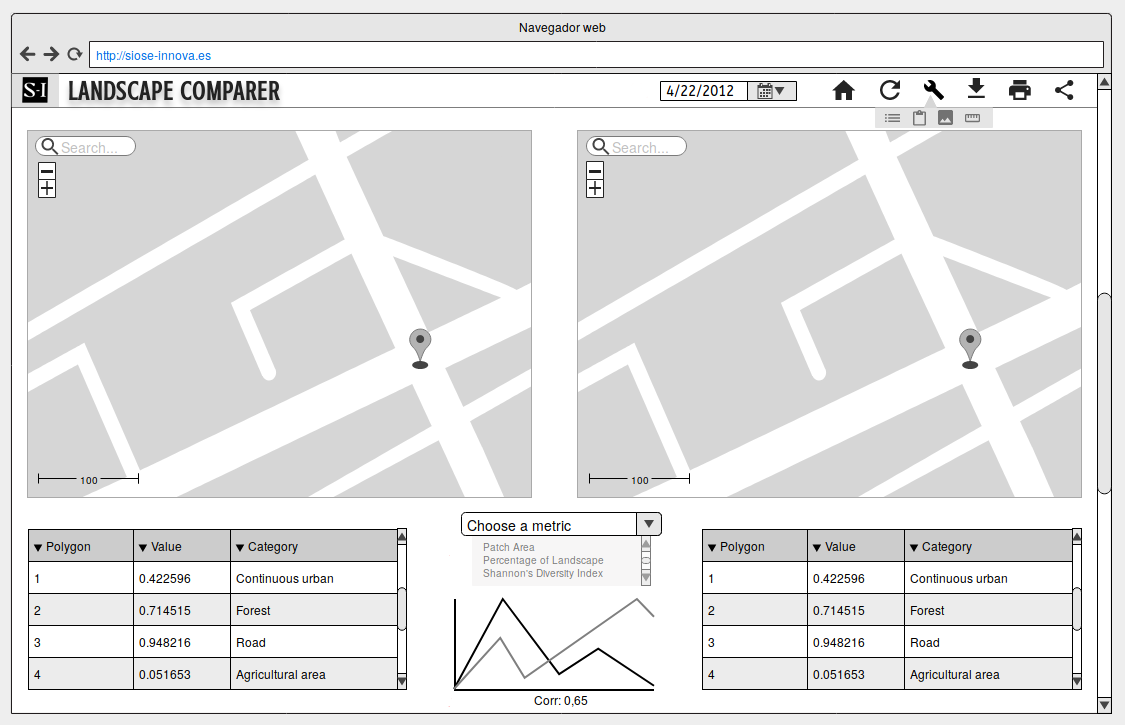
\includegraphics[width=\textwidth]{Prologo/Figs/visorweb.png}
\caption{Prototipo de un visor cartográfico para el análisis (comparación) de la estructura del paisaje a partir del SIOSE. La extensión sobre PostgreSQL/PostGIS desarrollada en este trabajo (\textit{pg\_landmetrics}) es la base para este tipo de aplicaciones. \label{fig:visorweb}}
\end{center}
\end{figure}

La extensión \textit{pg\_landmetrics} encapsula consultas SQL más complejas y \textbf{hace posible calcular múltiples métricas del paisaje en sentencias de una o muy pocas líneas}. Además, esta extensión se instala de un modo sencillo y \textbf{permite trabajar con bases de datos voluminosas} como la del SIOSE (millones de registros; Gigabytes de memoria; ver Tabla \ref{tab:datos}). 

Una cuestión que va más allá de los objetivos de este trabajo tiene que ver con el verdadero potencial de la plataforma de \textit{contenerización} con la que se ha desarrollado \textit{pg\_landmetrics}. Al tratarse de un \textit{software libre} y \textit{contenerizado} (ver capítulo \ref{chap:metod}), se facilita la distribución de esta aplicación a otros equipos (servidores y/o PCs), lo cual \textbf{aporta una escalabilidad que ningún entorno de escritorio puede lograr}. Es decir que a más usuarios del SIOSE, resultaría sencillo añadir nuevos servidores para realizar el análisis.

\subsection*{Estructura del trabajo}
Este trabajo se organiza en cuatro capítulos, a parte las referencias bibliográficas y los anexos. De un modo general, la estructura seguida es la siguiente:
\begin{itemize}
\item En el capítulo \ref{chap:intro} se revisa el uso de las bases de datos de ocupación del suelo y su papel en el análisis de la estructura del paisaje a partir de métricas de paisaje. Al final se presentan los objetivos generales y específicos de este trabajo.

\item En el capítulo \ref{chap:metod} se describen los conjuntos de datos, herramientas, plataformas tecnológicas y metodología seguida para diseñar e implementar una nueva extensión sobre PostgreSQL/PostGIS. La metodología incluye desde el trabajo colaborativo en varias plataformas de desarrollo, hasta las tareas diarias, la incorporación de funciones y la documentación de la extensión. Finalmente, se plantean una serie de experiencias computacionales para evaluar la extensión de acuerdo con los objetivos del trabajo.

\item En el capítulo \ref{chap:result} se detallan todos los resultados obtenidos, tanto en forma de código, como aquellos resultados obtenidos en un caso de estudio que simula una aplicación real (ver Figura \ref{fig:visorweb}).

\item Finalmente, en el capítulo \ref{chap:concl} se revisa el trabajo realizado para valorar cómo se han alcanzado los objetivos propuestos en la introducción. El capítulo termina por detallar los próximos pasos que seguirá el equipo de desarrollo para completar una extensión en \textit{fase de producción} (p. ej. un visor publicado desde una página web del IGN).
\end{itemize}



\end{prologo}

% ************************** Resumen *****************************
% Use `abstract' as an option in the document class to print only the titlepage and the abstract.

\begin{resumen}

La existencia de base de datos espaciales cada vez más amplias y voluminosas conlleva a distintos retos en el sentido de manejar y proporcionar un acceso ágil y directo de sus informaciones. La base de dados del Sistema de Información sobre Ocupación del Suelo de España (SIOSE) es un claro ejemplo de esta situación, al presentar informaciones de compleja codificación y decenas de millones de registros, exigiendo de sus usuarios una gran capacidad de procesamiento y almacenamiento.

Este trabajo se enmarca dentro de los objetivos propuestos por el Proyecto SIOSE-INNOVA que plantea dos líneas de trabajo, una de innovación técnica y otra aplicada, que buscan potenciar la usabilidad del SIOSE en distintos tipos de estudio.

Entre el gran número de aplicaciones posibles a partir de bases de datos como la del SIOSE, las métricas del paisaje son útiles para analizar la estructura y comportamiento del paisaje. Sin embargo, dada la gran diversidad de métricas, ningún programa permite calcular todas las métricas ni está pensado para trabajar con geodatabases tan complejas y voluminosas como es la del SIOSE la cual se refiere también a problemas de usabilidad.
 
El objetivo principal de este trabajo es crear una extensión sobre PostgreSQL/PostGIS capaz de calcular métricas de paisaje a partir de la base de datos del SIOSE, haciendo frente a los problemas de usabilidad. La pregunta central de este trabajo es si esta extensión será capaz de hacer frente a los mencionados problemas que afectan al SIOSE y geodatabases similares. 

El desarrollo de esta extensión, denominada \pgland{}, ha sido posible gracias al uso de herramientas de desarrollo colaborativo y plataformas de contenerización o virtualización de servicios. Han permitido establecer flujos de trabajo de integración continua e ir generando una extensión funcional capaz de calcular métricas de paisaje a partir del SIOSE-2011. Se han utilizado toda una variedad de técnicas de programación en bases de datos para que los usuarios sean capaces de calcular métricas de paisaje en sentencias de una o unas pocas líneas. Finalmente, para poner a prueba la extensión, se ha llevado a cabo una experiencia computacional sobre el SIOSE-2011 a partir de repetidas consultas de métricas. 

Este trabajo sirve para poner en valor el trabajo colaborativo basado en una serie de herramientas de control de versiones, contenerización y orquestación. Esta metodología facilitará enormemente a seguir añadiendo nuevas métricas y aplicar esta extensión a nuevos estudios relacionados con la estructura del paisaje.\\


\textbf{Palabras clave}: SIOSE, \textit{usabilidad}, métricas de paisaje, PostGIS, reproducibilidad, contenerización.


\end{resumen}

% ************************** Abstract *****************************
% Use `abstract' as an option in the document class to print only the titlepage and the abstract.

\begin{abstract}

The existence of increasingly large and voluminous spatial databases leads to different challenges in the sense of managing and providing an agile and direct access to their information. The database of the Information System on Land Occupation of Spain (SIOSE) is a clear example of this situation, when presenting information of complex coding and tens of millions of records, demanding from its users a great capacity for processing and storage. Among the large number of possible applications from databases such as the SIOSE, landscape metrics are useful for analyzing the structure and behavior of the landscape. Currently, there are many softwares designed to offer calculations and analysis of landscape patterns from databases of land occupation (FRAGSTATS, Patch Analyst, etc). However, no program can calculate all the metrics nor is it designed to work on current, more complex and voluminous geodatabases, which refers to the \textit{usability} problems related to the SIOSE. The main objective of this work is to create a PostgreSQL / PostGIS extension capable of calculating landscape metrics from the SIOSE database, dealing with \textit{usability} problems. The central question of this work is whether this extension will be able to cope with the aforementioned \textit{usability} problems that affect the SIOSE and other similar geodatabases.\\


\textbf{Key words}: SIOSE, \textit{usability}, landscape metrics, PostGIS, extension.


\end{abstract}

% *********************** Adding TOC and List of Figures ***********************
\tableofcontents

\listoffigures

\renewcommand{\listtablename}{Índice de tablas}
\renewcommand{\tablename}{Tabla}
\listoftables

\newpage
\addcontentsline{toc}{chapter}{Ejemplos de código}
\lstlistoflistings


% \printnomenclature[space] space can be set as 2em between symbol and description
%\printnomenclature[3em]

\printnomenclature

% ******************************** Main Matter *********************************
\mainmatter

 %!TEX root = ../thesis.tex
%*******************************************************************************
%*********************************** Introduccion *****************************
%*******************************************************************************

\chapter{Introducción}\label{chap:intro}

La interacción de los factores naturales y antrópicos es el origen de la estructura espacial compleja y heterogénea que presenta el paisaje \citep{Forman1986,Turner2001}. En las últimas décadas, la ecología del paisaje ha estudiado la configuración, el tamaño y la forma de los componentes que estructuran el territorio utilizando \textbf{métricas de paisaje} \citep{Aguilera2010}. Hoy en día, para estudiar la estructura del paisaje se dispone de \textbf{gran cantidad de información y herramientas}. 

En primer lugar, las bases de datos de ocupación del suelo, como por ejemplo el Sistema de Información de Ocupación del Suelo en España (SIOSE), representan el territorio de un modo adecuado para aplicar conceptos fundamentales como los de conectividad o diversidad del paisaje. Además, estas bases de datos aumentan progresivamente en riqueza semántica y resolución geométrica, por lo que \textbf{la información disponible no para de crecer}.

Complementariamente, también existe software específico o de carácter más general que facilita el cálculo de métricas del paisaje. Sin embargo, \textbf{ninguna de las aplicaciones encontradas es lo suficientemente escalable y extensible como para analizar grandes bases de datos de ocupación del suelo tan complejas como las actuales} (p.ej. SIOSE). 

Evidentemente, los problemas existentes al analizar las geodatabases actuales irá en aumento con la cada vez mayor disponibilidad de datos obtenidos a partir de imágenes de satélite o datos de campo. Este trabajo se enmarca en este contexto de creciente complejidad y busca \textbf{proponer herramientas más sencillas y eficientes en el cálculo de métricas del paisaje}.


\section{Estudio de la estructura del paisaje utilizando el SIOSE}\label{sec:siose}

\begin{graybox}
\begin{itemize}
\item El SIOSE es una valiosa \textbf{base de datos de ocupación del suelo} que contiene un gran volumen de información territorial de toda España.
\item Desde su aparición en 2005, SIOSE se ha convertido en un repositorio de referencia para sus homólogos europeos, llegando a ser un \textbf{modelo para la iniciativa EAGLE} (\textit{SIOSE europeo}). 
\item A pesar de su gran potencial, el SIOSE presenta ciertos problemas de \textit{usabilidad} debidos a su gran volumen y complejidad (p.ej. desde aplicaciones SIG de escritorio).
\end{itemize}
\end{graybox}


El Sistema de Información de Ocupación del Suelo en España (SIOSE) se lanzó en el año 2005 por la Dirección General del Instituto Geográfico Nacional de España (IGN)\footnote{\url{http://www.ign.es/web/ign/portal}} ante la necesidad de adquirir información más detallada a nivel nacional. El SIOSE está integrado en el Plan Nacional de Observación del Territorio (PNOT) con el objetivo de alcanzar una infraestructura de datos espaciales multidisciplinar. Este conjunto de datos va a ser un componente imprescindible para llevar a cabo los objetivos de este trabajo.

El SIOSE es una base de datos que recoge información de la ocupación del suelo de España en forma de malla continua de polígonos a partir de la fotointerpretación de imágenes. Cada polígono se especifica por dos componentes: la cobertura del suelo (\textit{Land Cover, LC}) se refiere a las características de la cubierta natural, como por ejemplo cuerpos de agua, bosques, superficies urbanas, zonas agrícolas, etc., y el uso del suelo (\textit{Land Use, LU})se define por las funciones socioeconómicas en el territorio, como por ejemplo uso industrial, residencial, forestal, agrícola, etc.

La escala de referencia es 1:25.000 y el sistema geodésico de referencia es European Terrestrial Reference System 1989 (ETRS89) con proyección Universal Transversa de Mercator (UTM). El tamaño mínimo de los polígonos depende del tipo de cobertura: 2 Ha para las zonas agrícolas, forestales y naturales, 1 Ha para las superficies artificiales y 0,5 Ha para agua, cultivos forzados, coberturas húmedas, playas, vegetación de ribera y acantilados. El SIOSE es un modelo orientado a objetos (entidad-relación) que describe los objetos, atributos y relaciones, y que permite la asignación de una o varias coberturas de suelo a un único polígono (datos semiestructurados). Cuando el polígono presente una única cobertura tendrá una \textit{cobertura simple}, pero cuando esté formado por dos o más coberturas tendrá una \textit{cobertura compuesta}, o también conocido como multietiqueta o \textit{multilabel} \citep{EquipoTecnicoNacionalSIOSE2015}. El hecho de que sea un modelo orientado a objetos, garantiza la compatibilidad y comparabilidad con otras bases de datos de ocupación del suelo como por ejemplo el \textit{Corine Land Cover (CLC)}.

El SIOSE tiene una proyección internacional ya que hay iniciativas similares en otros muchos países. Concretamente, el grupo EAGLE (Eionet Action Group on Land monitoring in Europe) tiene como objetivo solucionar la vigilancia de la tierra sobre la información europea de las fuentes de datos nacionales para una mejor integración y armonización a partir del concepto \textit{bottom-up}, además de facilitar el intercambio y comparación de datos entre países europeos \citep{Arnold2013}. Gracias a la iniciativa de EAGLE, el Instituto Geográfico Nacional de España (IGN) crea el SIOSE que se ha convertido en un repositorio de ocupación del suelo de referencia a nivel europeo \citep{EquipoTecnicoNacionalSIOSE2015}. Así pues, uno de los objetivos futuros del SIOSE es obtener una base de datos de ocupación del suelo europea para que resulte más fácil trabajar entre fronteras.

El análisis de la estructura del paisaje a partir de datos de usos y coberturas del suelo ha sido aplicado habitualmente desde diversas disciplinas y ámbitos de estudio. Por ejemplo, se han realizado estudios sobre:

\begin{itemize}
\item Medio Ambiente, hábitats naturales \citep{Gine2014,Hamilton2009,Hebeisen2008}\citep{GimenezFont2010,Lin2014,Brennan2005}.
\item Demografía, urbanismo y planificación del territorio \citep{Aguilera2011}, \citep{Blaschke1999,Jacquin2008,Tudor2014,Aguilera2010,Prastacos2017}
\item Infraestructuras, energía y transporte.
\item Dinámica de la ocupación del suelo \citep{VanderKwast2011,Dunk2011,Herold2002}, \citep{Roces-Diaz2014,Aguilera2012,Liu2016,Rodriguez-Rodriguez2017}
\end{itemize}

También se han realizado estudios sobre abandono agrícola \citep{Zaragozi2011} y otros sobre el riesgo de incendio asociado a nuevas formas de ocupación del suelo \citet{Vazquez2017}.

Los principales usuarios que trabajan con información sobre ocupación del suelo son la Administración General, gobiernos autonómicos, universidades, organismos de investigación, organismos europeos e internacionales, empresas públicas y privadas y, en menor medida, los usuarios particulares.

Todos estos usuarios del SIOSE se ven afectados por dos dificultades relacionadas con la \textit{usabilidad} de los datos: \textbf{el gran volumen de datos y la complejidad del modelo de datos}. La base de datos está formada por unos 2,5 millones de geometrías poligonales con sus coberturas de suelo. Este volumen de datos influye de manera importante en la capacidad de los usuarios para consultar o manejar esta información. La complejidad del modelo de datos es mayor que en bases de datos más tradicionales. El modelo SIOSE se compone de 85 clases, que forman un total de 820.632 casos de coberturas de suelo diferentes (simples y compuestas) \citep{FernandezVillarino2012}. Este nivel de complejidad del modelo de datos hace que el SIOSE sea dificil de utilizar por parte de usuarios que no conozcan el modelo o que no son especialistas en geodatabases. La gran cantidad de geometrías y la complejidad de las clasificaciones dificultan gestionar esta información mediante a aplicaciones SIG (Sistemas de Información Geográfica) convencionales, ya que se puede llegar a superar la capacidad de éstas. Todo ello hace que sea necesario estudiar otras nuevas tecnologías \citep{NavarroCarrion2016}.

En el proyecto SIOSE-INNOVA se plantea investigar y proponer soluciones para los problemas de \textit{usabilidad} descritos por el mismo equipo de desarrollo del SIOSE en \citet{FernandezVillarino2012}. Durante el desarrollo de este proyecto de tres años de duración, se quieren alcanzar los siguientes objetivos específicos:
\begin{enumerate}
\item Crear un marco de experimentación reproducible y fácilmente utilizable por un gran número de usuarios.
\item Analizar las necesidades y rendimiento de distintas tecnologías de bases de datos NoSQL para la explotación del SIOSE.
\item Desarrollar e implementar un nuevo modelo de datos auxiliar que permita extender las posibilidades de análisis del SIOSE con técnicas de \textit{Big Data} o \textit{Data Mining}.
\item Evaluar la \textit{usabilidad} de los datos SIOSE en distintas plataformas tecnológicas, mediante su aplicación en casos de uso reales en los que utilizar datos de ocupación del suelo resulte esencial.
\end{enumerate}


\section{Métricas de paisaje y software que las calcula}\label{sec:metrica}

\begin{graybox}
\begin{itemize}
\item Las \textbf{métricas de paisaje} son métodos cuantitativos que sirven para analizar la estructura del paisaje y otros fenómenos (p.ej. evolución del paisaje, conectividad de ecosistemas, entre otros).
\item FRAGSTATS, Conefor Sensinode, Patch Analyst, entre otros, son aplicaciones de escritorio muy utilizadas para el cálculo de métricas del paisaje. No obstante, \textbf{no hay ninguna aplicación} que sea fácilmente \textbf{escalable y extensible} como para realizar análisis sobre una geodatabase similar a la del SIOSE.
\end{itemize}
\end{graybox}

El paisaje comprende la interacción entre los factores naturales y artificiales, causantes de la evolución y estructura compleja y heterogénea que presenta el suelo. Por este motivo, se utilizan las métricas de paisaje como técnica/metodología para el estudio del paisaje y otros fenómenos. Las métricas son métodos cuantitativos que funcionan como algorítmos matemáticos encargados de aportar resultados numéricos \citep{Gine2014}.

Hay cientos de métricas de paisaje, correlacionadas entre sí, pero no todas las métricas tendrán significado en todos los contextos y/o estudios. Algunas de las investigaciones que utilizan las métricas de paisaje son aquellas relacionadas con biodiversidad, hábitats, aplicaciones de agua, cambios de suelo, estructura urbana, infraestructura vial, riesgos naturales, estética del paisaje, planificación territorial, entre otros \citep{Uuemaa2009}. Por ejemplo, en \citet{Uuemaa2017} se investigan aquellas métricas que parecen estar más relacionadas con los estudios forestales para explicar las relaciones entre los procesos ecológicos y los patrones espaciales existentes en una zona. \textbf{Esto indica que los investigadores necesitarán calcular un gran número de métricas para cada paisaje y después aplicar algún criterio de selección para determinar cuales son las más descriptivas en cada caso.}

Las métricas de paisaje se pueden calcular a partir de aplicaciones de escritorio. En \citet{Zaragozi2012} se establece una comparativa entre \textbf{programas específicos} para el cálculo de métricas del paisaje, destacando entre ellos FRAGSTATS \citep{McGarigal1994,McGarigal2015}. Por otro lado, hay otros programas como Conefor Sensinode \citep{Saura2009}, Patch Analyst, varios módulos de GRASS GIS, LecoS \citep{Jung2016}, ZonalMetrics \citep{Adamczyk2017}, entre otros. Evidentemente, esta lista no puede estar completa, ya que hay muchos otros programas que pueden calcular un número de métricas variable según un gran número de factores.

Existen muchos otros programas especializados que permiten el cálculo de este tipo de métricas/índices pero no siempre tiene que ser una aplicación específica que las calcule. También es posible calcular facilmente determinadas métricas con \textbf{herramientas típicas de un SIG} de escritorio (calculadora de campos y/o calculadora raster, entre otras posibilidades).

En cualquier caso, no hay ninguna aplicación escalable y extensible capaz de realizar análisis sobre bases de datos de ocupación del suelo tan voluminosas y complejas como lo es la del SIOSE.


\section{Objetivos}\label{sec:objetivos}

El principal objetivo de este trabajo es \textbf{desarrollar una extensión (PostgreSQL/PostGIS) que facilite el cálculo de métricas de paisaje}. Se quiere facilitar la realización de consultas y permitir el manejo de bases de datos voluminosas como lo es la del SIOSE \textit{actual}. 

Previsiblemente, las bases de datos de ocupación del suelo no harán sino aumentar en volumen y complejidad, por lo que si hoy en día existen los mencionados problemas de usabilidad del SIOSE, estos no harán sino ir a más. Así el trabajo desarrollado tendrá continuidad en el tiempo.

Enlazando con el objetivo principal de este trabajo surgen una serie de objetivos más específicos relacionados con la metodología planteada en el proyecto SIOSE-INNOVA. En este sentido, se han considerado los siguientes \textbf{objetivos específicos}:
\begin{enumerate}
\item Aplicar herramientas de \textbf{desarrollo colaborativo} para trabajar con los otros investigadores del proyecto SIOSE-INNOVA.
\item Validar sistemáticamente que la extensión desarrollada funciona correctamente (\textit{integración continua}; tests de unidad).
\item Aplicar las prácticas y estándares de desarrollo más novedosos.
\item Realizar un \textbf{experimento con una geodatabase de usos del suelo de gran complejidad y volumen}, como es el SIOSE (2011).
\item Adquirir \textbf{nuevos conocimientos} a lo largo de este trabajo sobre herramientas de desarrollo colaborativo, contenerización y orquestación, lenguajes de programación y lenguajes procedurales.
\item Poner en práctica los \textbf{conocimientos adquiridos durante el aprendizaje en el \textit{máster}} de las distintas asignaturas impartidas sobre teoría e implementación de bases de datos, lenguajes de programación, software libre, aplicaciones infográficas y análisis espacial.
\end{enumerate}






%!TEX root = ../thesis.tex
%*******************************************************************************
%****************************** Metodologia *********************************
%*******************************************************************************


\chapter{Metodología}\label{chap:metod}

Este trabajo aplica una metodología de \textbf{integración continua y desarrollo colaborativo} de acuerdo con los objetivos del proyecto SIOSE-INNOVA y con un marco de trabajo actual aplicado tanto en el Laboratorio de Geomática de la Universidad de Alicante como por otras empresas conocidas del sector (CARTO, Geographica, entre otros). En \citet{Zaragozi2017} se presentan distintos flujos de trabajo basados en esta metodología los cuales están muy relacionados con lo que se presenta en este capítulo.


\section{Integración continua y desarrollo colaborativo}

\begin{graybox}
\begin{itemize}
\item El trabajo colaborativo se ha coordinado utilizando \textit{Git} que es el sistema de \textbf{control de versiones} más popular de los últimos años (p.ej. utilizado en , PostGIS, QGIS, CARTO y decenas de proyectos ESRI, entre muchos otros).
\item La \textbf{contenerización o \textit{dockers}} es una novedosa tecnología para la virtualización de software/servicios, frente a la virtualización de sistemas operativos (p.ej. máquinas virtuales). La orquestación de \textit{dockers} permite organizar complejos sistemas de información con muchas facilidades.
\item PostgreSQL/PostGIS es la \textit{geodatabase libre} más potente del mercado, destacando por sus opciones de \textbf{extensibilidad} (p.ej. PostGIS en sí misma es una extensión de PostgreSQL).
\end{itemize}
\end{graybox}



\subsection{Control de versiones}


\begin{itemize}
\item\textbf{Git}: 
\item\textbf{GitHub}: 
\end{itemize}



\begin{figure}
\begin{center}
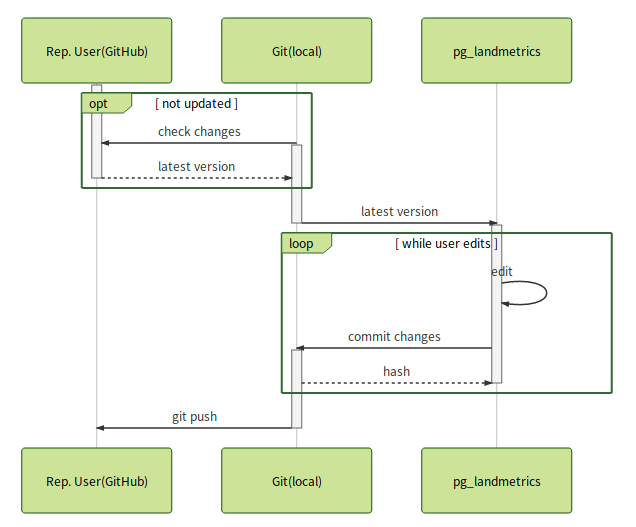
\includegraphics[width=0.9\textwidth]{Metodologia/Figs/diary.png}
\caption{Flujo de proceso de actualización de ficheros. \label{fig:diary}}
\end{center}
\end{figure}



\begin{figure}
\begin{center}
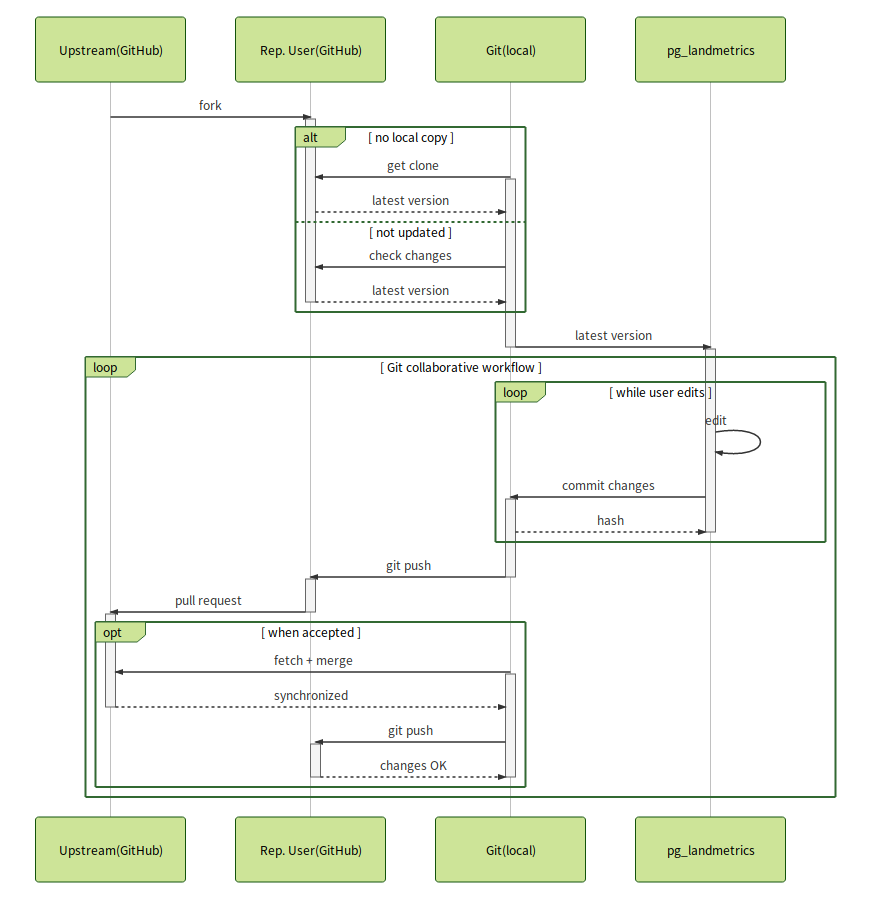
\includegraphics[width=0.9\textwidth]{Metodologia/Figs/pullrequest.png}
\caption{Flujo de proceso de trabajo colaborativo entre repositorios. \label{fig:pullrequest}}
\end{center}
\end{figure}


\subsection{Contenerización y orquestación de servicios}





Se han utilizado los siguientes elementos:
\begin{itemize}
\item\textbf{Docker}: 
\item\textbf{Docker Hub}: 
\item\textbf{Docker-compose}: 
\end{itemize}




\begin{figure}
\begin{center}
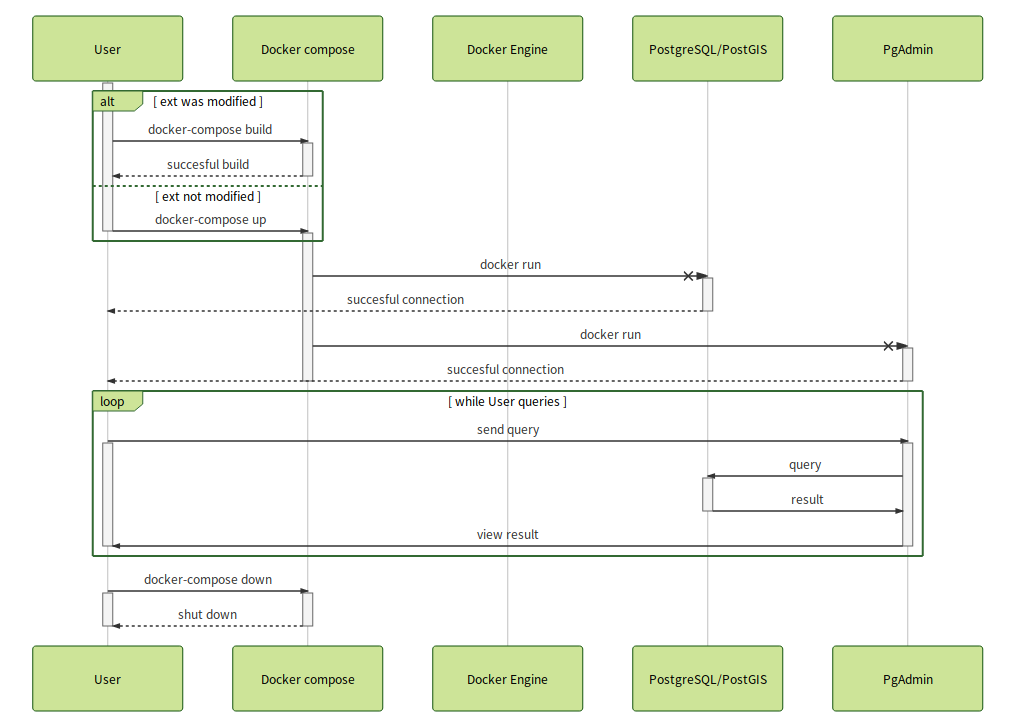
\includegraphics[width=\textwidth]{Metodologia/Figs/ci.png}
\caption{Flujo de proceso de integración continua. \label{fig:ci}}
\end{center}
\end{figure}


\subsection{Extensibilidad}



\begin{itemize}
\item\textbf{PostgreSQL/PostGIS}: 
\end{itemize}

\subsection{Aplicaciones}



\begin{itemize}
\item\textbf{PgAdmin4}: 

\begin{figure}
\begin{center}
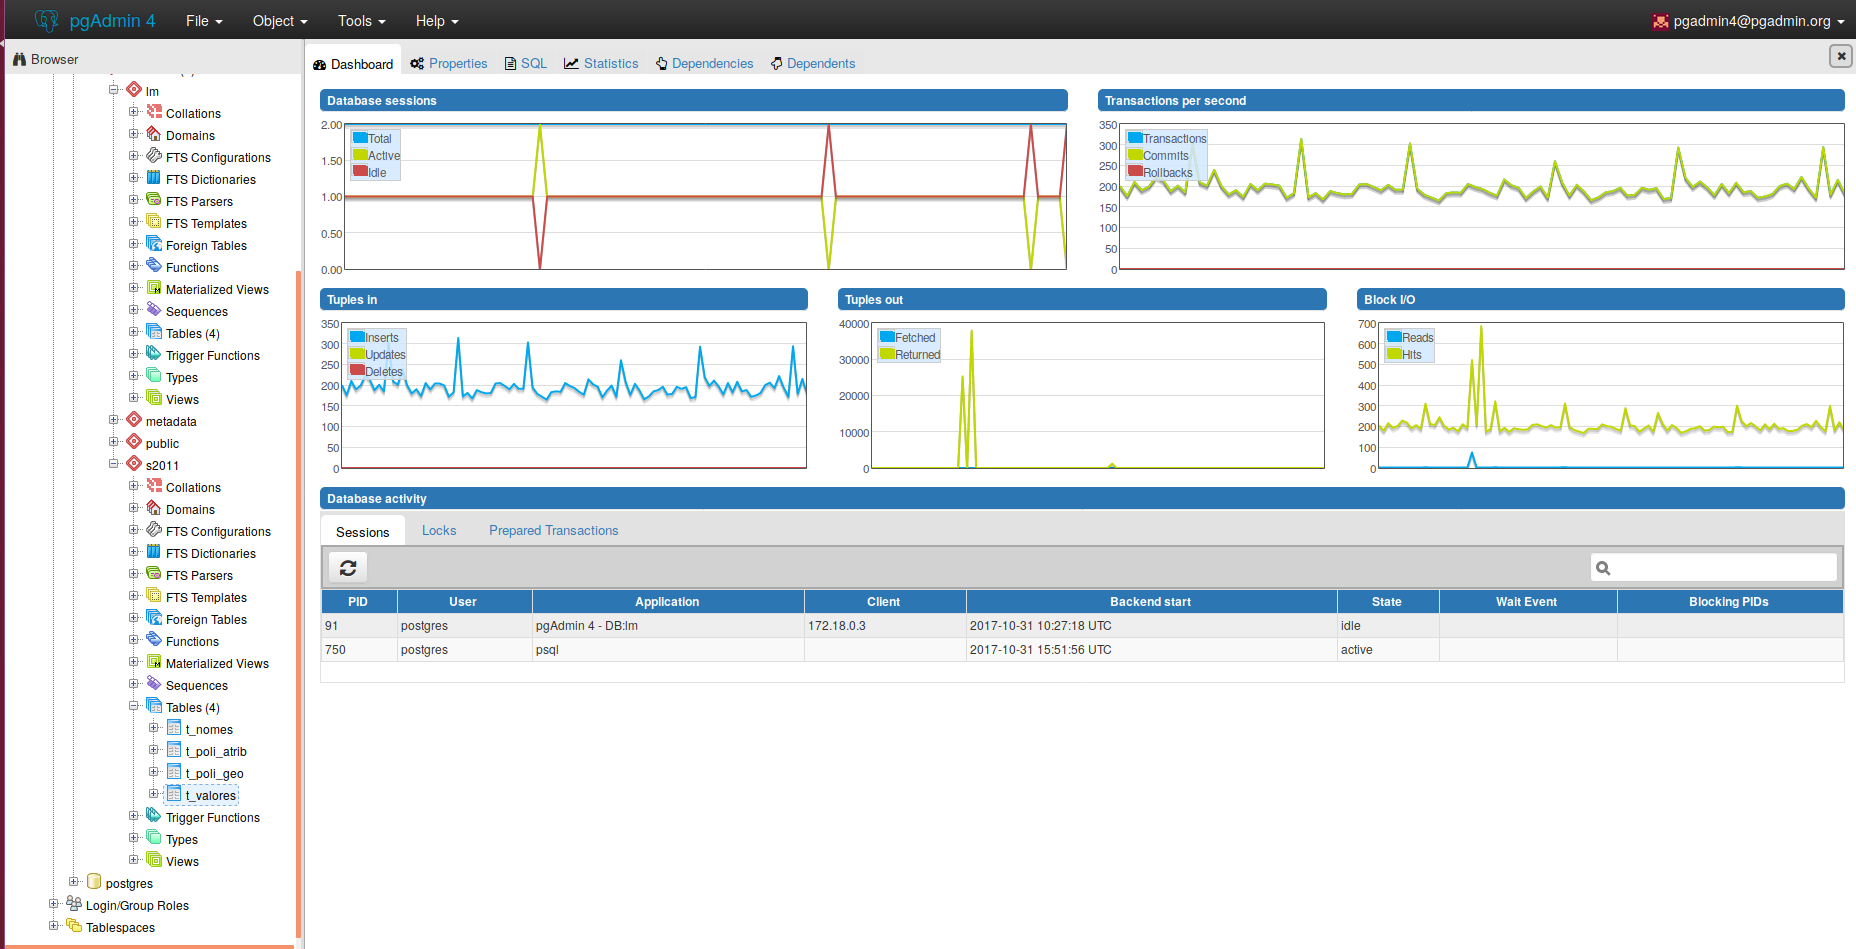
\includegraphics[width=\textwidth]{Metodologia/Figs/carga-siose-2011.png}
\caption{Flujo de proceso de integración continua. \label{fig:carga}}
\end{center}
\end{figure}

\item\textbf{QGIS 2.18}: 
\end{itemize}

\section{Conjunto de datos}

\begin{graybox}
\begin{itemize}
\item En este trabajo se han utilizado dos conjuntos de datos, \textbf{un paisaje de ejemplo y el SIOSE de 2011 completo}, para poner a prueba la extensión \textit{pg\_landmetrics} propuesta en los objetivos.
\end{itemize}
\end{graybox}

Antes de escoger las métricas de paisaje adecuadas, se han utilizado dos conjuntos de datos, un paisaje de ejemplo y el SIOSE 2011, para someter a prueba la extensión \textit{pg\_landmetrics}.

En el paisaje de ejemplo se han digitalizado todos los polígonos que lo comprenden. Se ha querido obtener un paisaje lo menos complejo posible para comprobar de manera más fácil si las métricas de paisaje funcionan correctamente. Para la elaboración de este paisaje se han utilizado las herramientas de geoproceso y edición de la aplicación de escritorio QGIS 2.18. 

Este paisaje se ha elaborado con escala de referencia 1:50.000 en dos sistemas geodésicos de referencia: European Terrestrial Reference System 1989 (ETRS89) y World Geodetic System 84 (WGS84), para comprobar que las métricas de paisaje funcionan desde una geometría o desde unas coordenadas geográficas. En cuanto a sus características técnicas, 



\begin{figure}
\begin{center}
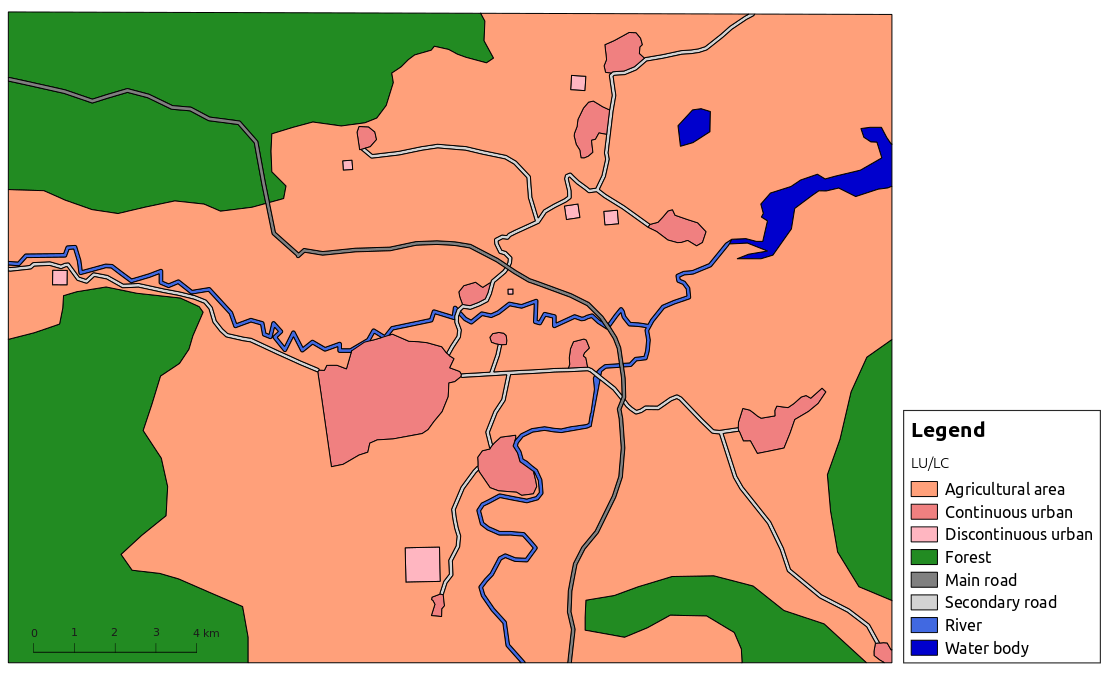
\includegraphics[width=\textwidth]{Metodologia/Figs/land_test.png}
\caption{Uso y cobertura del suelo del paisaje de ejemplo. \label{fig:lan_test}}
\end{center}
\end{figure}



% Please add the following required packages to your document preamble:
% \usepackage{booktabs}
% \usepackage{multirow}
\begin{table}[]
\centering
\caption{Características de los conjuntos de datos utilizados\label{tab:datos}}
\begin{tabular}{@{}llll@{}}
\toprule
\textbf{Tipo}               & \textbf{Tablas} & \textbf{Filas} & \textbf{Tamaño total} \\ \midrule
\multirow{4}{*}{SIOSE-2011} & t\_nomes        & 36.790.972     & 6116 MB               \\
                            & t\_poli\_atrib  & 2.562.800      & 451 MB                \\
                            & t\_poli\_geo    & 2.562.800      & 3981 MB               \\
                            & t\_valores      & 10.932.639     & 1041 MB               \\ \midrule
\multirow{4}{*}{Grids}      & g25k            & 756            & 232,3 kB              \\
                            & g50k            & 192            & 57,8 kB               \\
                            & g100k           & 48             & 13,8 kB               \\
                            & g500k           & 2              & 677bytes              \\ \midrule
\multirow{2}{*}{Sample}     & sample\_25830   & 51             & 122,6 kB              \\
                            & sample\_4326    & 51             & 122,5 kB               \\ \bottomrule
\end{tabular}
\end{table}





\section{Selección de métricas}

\begin{graybox}
\begin{itemize}
\item El número potencial de métricas del paisaje es indeterminado y depende de muchos factores (p.ej. objetivos del estudio, modelos de datos como \textit{raster/vector} o en red, niveles de agregación y/o escala, etc).
\item Resulta esencial determinar unas \textbf{métricas representativas} para esta primera propuesta.
\end{itemize}
\end{graybox}

Como se indica en la sección \ref{sec:metrica}, existen cientos de métricas de paisaje que no siempre tienen significado para todas las aplicaciones de estudio ya que dependen de muchos factores, como por ejemplo los objetivos del estudio, el modelo de datos, la escala, nivel de agregación etc. Por este mismo motivo y según los objetivos específicados en este trabajo y en el proyecto SIOSE-INNOVA, se han seleccionado unas determinadas métricas de paisaje.

En la tabla \ref{tab:listmetricas} se aprecian las métricas, acompañadas por su abreviatura, que se han escogido divididas en tres niveles de agregación: a nivel polígono (\textit{patch}), nivel categoría (\textit{class}) y nivel paisaje (\textit{landscape}). Para ello se ha seleccionado un número equitativo entre los niveles de agregación. Además, se han querido escoger algunas métricas que calculen operaciones simples como por ejemplo el área o perímetro, y por otro lado, métricas cuyos cálculos sean más complejos como por ejemplo la distancia del vecino más próximo o la densidad, entre otros.

% Please add the following required packages to your document preamble:
% \usepackage{multirow}
\begin{table}[]
\centering
\caption{Listado de métricas de paisaje disponibles en la extensión.}
\label{tab:listmetricas}
\begin{tabular}{lll}
\hline
\textbf{Nivel}             & \textbf{Métrica}                     & \textbf{Abreviatura} \\ \hline
\multirow{8}{*}{Patch}     & Patch Area                           & AREA                 \\
                           & Patch Perimeter                      & PERIM                \\
                           & Perimeter-Area-Ratio                 & PARA                 \\
                           & Shape Index                          & SHAPE                \\
                           & Core Area                            & CORE                 \\
                           & Number of Core Areas                 & NCORE                \\
                           & Core Area Index                      & CAI                  \\
                           & Euclidean Nearest Neighbour Distance & ENN                  \\ \hline
\multirow{8}{*}{Class}     & Total (Class) Area                   & CA                   \\
                           & Percentage of Landscape              & PLAND                \\
                           & Total Edge                           & TE                   \\
                           & Edge Density                         & ED                   \\
                           & Total Core Area                      & TCA                  \\
                           & Core Area Percentage of Landscape    & CPLAND               \\
                           & Number of Patches                    & NP                   \\
                           & Patch Density                        & PD                   \\ \hline
\multirow{9}{*}{Landscape} & Total Area                           & TA                   \\
                           & Total Edge                           & TE                   \\
                           & Edge Density                         & ED                   \\
                           & Number of Patches                    & NP                   \\
                           & Patch Density                        & PD                   \\
                           & Patch Richness                       & PR                   \\
                           & Patch Richness Density               & PRD                  \\
                           & Shannon's Diversity Index            & SHDI                 \\
                           & Simpson's Diversity Index            & SHIDI                \\ \hline
\end{tabular}
\end{table}


\section{Implementación/desarrollo de funciones en PostgreSQL}

\begin{graybox}
\begin{itemize}
\item Los desarrollos en PostgreSQL se pueden realizar en lenguajes de programación como ANSI C, SQL y/o distintos lenguajes procedurales (p.ej. PLpgSQL, PL/R, PL/Python, entre muchos otros), \textbf{dependiendo de las necesidades}.
\end{itemize}
\end{graybox}


\lstset{caption=Crear una función para calcular el IDW (I),label= IDW1}
\begin{SQL}
SELECT St_Area(geom)/10000 FROM sample_patches_25830;
SELECT St_Area(geom)/10000 FROM sample_patches_4326;
\end{SQL}

\lstset{caption=Crear una función para calcular el IDW (I),label= IDW1}
\begin{SQL}
SELECT SUM(St_Area(geom))/10000, category FROM sample_patches_25830 GROUP BY category;
SELECT SUM(St_Area(geom))/10000, category FROM sample_patches_4326 GROUP BY category;
\end{SQL}

\lstset{caption=Crear una función para calcular el IDW (I),label= IDW1}
\begin{SQL}
SELECT SUM(St_Area(geom)) FROM sample_patches_25830;
SELECT SUM(St_Area(geom)) FROM sample_patches_4326;
\end{SQL}


\lstset{caption=Crear una función para calcular el IDW (I),label= IDW1}
\begin{SQL}
SELECT St_Distance(p1.geom, p2.geom) 
FROM sample_patches_25830 AS p1, sample_patches_25830 AS p2
WHERE p1.id = 1 AND p1.id <> p2.id AND p2.category= "category"
ORDER BY St_Distance (p1.geom, p2.geom)
LIMIT 1;

SELECT St_Distance(p1.geom, p2.geom) 
FROM sample_patches_4326 AS p1, sample_patches_4326 AS p2
WHERE p1.id = 1 AND p1.id <> p2.id AND p2.category= "category"
ORDER BY St_Distance (p1.geom, p2.geom)
LIMIT 1;
\end{SQL}

\lstset{caption=Crear una función para calcular el IDW (I),label= IDW1}
\begin{SQL}
SELECT SUM(St_Area(St_Buffer(geom, -100)))/10000 FROM sample_patches_25830 GROUP BY category;
SELECT SUM(St_Area(St_Buffer(geom, -100)))/10000 FROM sample_patches_4326 GROUP BY category;
\end{SQL}

\lstset{caption=Crear una función para calcular el IDW (I),label= IDW1}
\begin{SQL}
SELECT SUM(St_Perimeter(geom)/St_Area(geom))*10000 FROM sample_patches_25830;
SELECT SUM(St_Perimeter(geom)/St_Area(geom))*10000 FROM sample_patches_4326;
\end{SQL}


\lstset{caption=Crear una función para calcular el IDW (I),label= IDW1}
\begin{SQL}
SELECT (p_corearea(geom, 50)).value FROM sample_patches_25830;
SELECT (p_corearea(geom, 50)).value FROM sample_patches_4326;
\end{SQL}

\lstset{caption=Crear una función para calcular el IDW (I),label= IDW1}
\begin{SQL}
SELECT c_totalarea(geom,category) FROM sample_patches_25830;
SELECT c_totalarea(geom,category) FROM sample_patches_4326;
\end{SQL}




\section{Documentación de la extensión}

\begin{graybox}
\begin{itemize}
\item Una parte fundamental de esta metodología es la \textbf{documentación} del desarrollo y uso de la extensión. 
\item Una buena documentación con ejemplos facilitará el cálculo de métricas del paisaje en grandes repositorios, \textbf{sobretodo para aquellos usuarios con menos experiencia} en PostgreSQL/PostGIS.
\end{itemize}
\end{graybox}

La documentación del desarrollo y uso de la extensión es una de las partes más importante de la metodología de este trabajo. Una buena documentación facilita la aplicación de todas las medidas necesarias para llevar a cabo el funcionamiento de la extensión a cualquier usuario, sobretodo a aquellos menos expertos en la materia. Así pues, se han aplicado los siguientes lenguajes de marcado:

\begin{itemize}
\item\textbf{Markdown}\footnote{\url{https://github.com/adam-p/markdown-here/wiki/Markdown-Cheatsheet}} es un lenguaje ligero que permite una escritura sencilla y de fácil lectura usando texto plano. Se ha utilizado para documentar el usp de la extensión.
\item\textbf{TeX}\footnote{\url{https://www.latex-project.org/}} es el lenguaje que se utiliza en el sistema de textos LaTeX y que crea documentos con una alta calidad tipográfica. Desde hace tiempo este lenguaje se emplea por un gran número de usuarios para escribir artículos o libros científicos. Para trabajar con este lenguaje, se ha utilizado la aplicación Texmaker y se ha utilizado para escribir este trabajo.
\item\textbf{Scalable Vector Graphics (SVG)}\footnote{\url{https://www.w3schools.com/graphics/svg_intro.asp}} es un lenguaje capaz de crear gráficos basados en vectores escalables de alta calidad de resolución. A partir de este lenguaje se ha desarrollado una función capaz de representar gráficos vectoriales a partir de las geometrías de cualquier geodatabase (ver en el anexo \ref{anex:svg}).
\item\textbf{Mermaid}\footnote{\url{https://mermaidjs.github.io/}} es un lenguaje que genera gráficos a partir de texto mediante JavaScript. Se han generado desde diagramas de flujo hasta diagramas de secuencia y de Gantt.
\end{itemize}

%!TEX root = ../thesis.tex
%*******************************************************************************
%****************************** Third Chapter **********************************
%*******************************************************************************
\chapter{Resultados y Discusión}\label{chap:result}

\begin{graybox}
\begin{itemize}
\item El principal resultado de este trabajo es la extensión pg\_landmetrics, en la cual se ha colaborado en un importante porcentaje de funcionalidades (\textit{commits}).
\item Las métricas implementadas en forma de funciones se han validado sistemáticamente para asegurar que devuelven el resultado correcto.
\item Se ha desarrollado un caso de uso completo basado en la aplicación propuesta en la introducción (ver Figura \ref{fig:visorweb}) con el que se han obtenido resultados prometedores (\textit{usabilidad} y volumen).
\end{itemize}
\end{graybox}


En este capítulo se presentan los resultados de este trabajo siguiendo una secuencia lógica y utilizando  figuras que ayuden a \textbf{visualizar cómo \textit{pg\_landmetrics} se integra en una aplicación como la descrita en la figura \ref{fig:visorweb}.}

Los resultados de este trabajo son prometedores y apuntan a que sí que se podrían publicar servicios de consulta, cómo el cálculo de las métricas del paisaje, a partir de la base de datos del SIOSE u otras de un volumen o complejidad similares.

En este capítulo también se destacan los  aspectos más novedosos y relevantes de este trabajo, así como las implicaciones de carácter práctico.

En la subsección \ref{sec:pglandmetrics} se describen las aportaciones realizadas al proyecto SIOSE-INNOVA y que corresponden al grueso del presente trabajo. A continuación, en la subsección \ref{sec:caso_uso} se presentan los resultados de un caso de uso o experiencia computacional en el que se ha puesto a prueba la extensión desarrollada. Entre los objetivos de este trabajo era importante permitir que los usuarios del SIOSE calculasen métricas de una manera sencilla e intuitiva, pero también que pudiesen manejar un gran volumen de datos, cosa que en otras aplicaciones muy conocidas no es posible (ver capítulo \nameref{chap:intro}).

\section{pg\_landmetrics \label{sec:pglandmetrics}}

Una parte importante de este trabajo ha consistido en aprender a colaborar en un equipo de desarrolladores de geodatabases. En la metodología de integración continua aplicada en el Laboratorio de Geomática de la Universidad de Alicante resulta relativamente sencillo hacer un repaso del trabajo realizado en cada fase del proyecto.

El uso de un software de control de versiones como Git y la gestión del proyecto en la plataforma GitHub, hacen posible seguir y analizar las aportaciones que los miembros del proyecto SIOSE-INNOVA han hecho en la extensión \textit{pg\_landmetrics}.

La plataforma GitHub ofrece numerosas estadísticas del trabajo de cada usuario y también de la vitalidad de cada proyecto. Por ejemplo, en la figura \ref{fig:contrib} se puede ver un diagrama de tipo \textit{calendar heatmap} extraido de GitHub, en el que se aprecia el número total de aportaciones al proyecto (\textit{commits}). 

\begin{figure}
\begin{center}
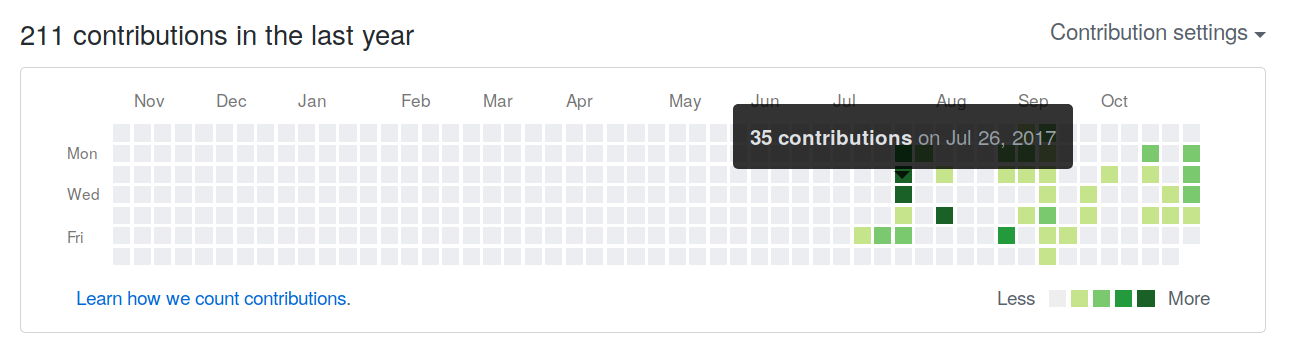
\includegraphics[width=\textwidth]{ResultadosyDiscusion/Figs/contributions.png}
\caption{Calendario de actividad y contribuciones de este trabajo al proyecto \textit{pg\_landmetrics} (\textit{heatmap calendar}). \label{fig:contrib}}
\end{center}
\end{figure}

Siguiendo con la figura \ref{fig:contrib}, los colores más intensos indican días de una mayor actividad, siendo el día 26 de julio el día en el que más aportaciones se realizó. Un numero tan grande de aportaciones es normal en la puesta en marcha de un proyecto de este tipo y en particular fue el día en el que se incorporaban sentencias SQL que habían sido testeadas en dias anteriores. Según la complejidad de las métricas o las funciones a desarrollar, hay días con una menor actividad y, en aquellos casos más problematicos, también hay días en los que los desarrollos los hacían otros miembros del equipo y había tiempo de preparar conjuntos de datos de ejemplo, preparar documentación o trabajar en la redacción del presente trabajo.

En total se ha contribuido al proyecto con 211 aportaciones, que posteriormente han sido aceptadas en la mayoría de los casos. El proyecto oficial únicamente muestra 209 contribuciones, pero ambas cifras no están directamente relacionadas. Hay que tener en cuenta que las acciones de \textit{pull request} explicadas en la figura \ref{fig:pullrequest} de la metodología suelen empaquetar varias actualizaciones o \textit{commits} que en el repositorio oficial aparecen como una única aportación. GitHub permite analizar el trabajo y la contribución de cada miembro del equipo de un modo muy minucioso.

El control de versiones sirve para recuperar un punto de trabajo anterior o también para supervisar cómo se ha ido desarrollando un trabajo. Aproximadamente, a partir de la figura \ref{fig:contrib} y otras similares es posible reconstruir las fases principales en que se desarrolló este trabajo. En julio se hizo una revisión bibliográfica y se aprendió a utilizar las herramientas vistas en la metodogía. A finales de julio se seleccionaron y se crearon consultas SQL para calcular la mayoría de las métricas. En agosto se creó un conjunto de datos de ejemplo y se validaron los resultados de cada consulta. En septiembre se convirtieron las consultas en funciones simples y, dado que no todas las métricas se podían implementar del mismo modo, en octubre se modificaron varias funciones para convertirlas en funciones de agregación. Finalmente, en noviembre se realizó el experimento computacional cuyos resultados se muestra en la sección \ref{sec:caso_uso}.

En el diagrama de red de GitHub (ver figura \ref{fig:network}) se puede visualizar el trabajo colaborativo desarrollado desde el principio hasta la realización de la experiencia computacional presentada en este trabajo. Se trata de un diagrama dinámico en el cual se puede consultar el contenido de cada contribución, ya sea la creación de nuevas funciones o cambios. En la figura \ref{fig:network} se pueden ver varios \textit{commits} por parte de distintos colaboradores, una operación de \textit{pull upstream}, cuatro operaciones \textit{push} y una serie de contribuciones propias que aún no habían sido aceptadas por el equipo del proyecto SIOSE-INNOVA. Los colores de las líneas ayudan a interpretar mejor este tipo de diagramas:

\begin{itemize}
\item La línea negra muestra los \textit{commits} integrados en el repositorio oficial.
\item Las líneas verdes y azules se refieren a aportaciones de este trabajo que finalmente fueron aceptadas por el equipo del SIOSE-INNOVA.
\item La línea morada hace referencia a las últimas funciones creadas, pendientes de aceptación al término de este trabajo.
\end{itemize}

\begin{figure}
\begin{center}
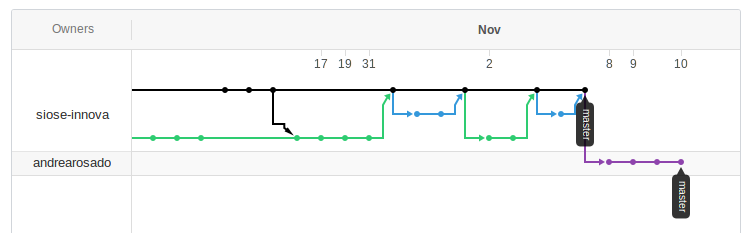
\includegraphics[width=\textwidth]{ResultadosyDiscusion/Figs/network.png}
\caption{Diagrama de red de GitHub.  \label{fig:network}}
\end{center}
\end{figure}

En cuanto a los resultados concretos de este trabajo, se han desarrollado varias funciones sobre PostgreSQL/PostGIS que calculan métricas del paisaje de distintos tipos. Todas las funciones se han creado por duplicado (\textit{funciones sobrecargadas}) para trabajar con sistemas de coordenadas planas y con coordenadas geográficas. Esta decisión tiene que ver con que en bases de datos tan voluminosas como la del SIOSE, en ocasiones será necesario realizar cálculos con polígonos que se encuentren muy distantes, llegando incluso a representarse en usos o sistemas de referencia espacial distintos. El uso de coordenadas esféricas permite trabajar con una geodatabase sin preocuparse de este tipo de problemas, pero a cambio de poder utilizar un número menor de funciones de PostGIS. No obstante, resulta que todas las métricas seleccionadas a partir de la documentación de FRAGSTATS han podido ser calculadas partiendo del tipo \textit{geography} de PostGIS. Esto hace que las operaciones con el SIOSE resulten más sencillas si no es necesario dividir la base de datos por usos o comunidades autónomas.

En la tabla \ref{tab:metrics-ext} se listan todas las métricas del paisaje implementadas en la extensión. Los colores indican si la métrica se ha podido desarrollar como una función SQL simple o si por el contrario ha sido necesario crear una función de agregación (combinación de varias funciones). 

En esta tabla de resumen también se puede ver que prácticamente todas las consultas se podían calcular manualmente (independientemente de la dificultad) salvo la distancia euclídea al vecino más próximo (ENN; Euclidean Nearest Neighbour Distance). Esta métrica implica numerosos cálculos de distancia entre polígonos, el uso de índices espaciales y la aplicación de una serie de filtros. Evidentemente, el calculo del ENN resultaría muy trabajoso si no se utiliza ningún lenguaje de programación. La consulta SQL para el ENN se realizó de un modo más o menos sencillo. Sin embargo, su implementación como función SQL de agregación está aún siendo revisada por el equipo del SIOSE-INNOVA.

Las métricas marcadas como pendientes de aceptación en la tabla \ref{tab:metrics-ext} devuelven el resultado correcto con el paisaje de ejemplo descrito en este trabajo, por lo que \textbf{es de esperar que pronto pasen a formar parte del repositorio oficial de \textit{pg\_landmetrics}}.


% Please add the following required packages to your document preamble:
% \usepackage{booktabs}
% \usepackage[table,xcdraw]{xcolor}
% If you use beamer only pass "xcolor=table" option, i.e. \documentclass[xcolor=table]{beamer}
\begin{table}[]
\centering
\caption{Listado de las métricas de paisaje disponibles en la extensión, según su nivel de complejidad y si han sido aceptadas en el repositorio oficial.}
\label{tab:metrics-ext}
\begin{tabular}{@{}lcccl@{}}
\toprule
\textbf{Métrica} & \textbf{Manual/QGIS} & \textbf{Consulta SQL} & \textbf{\textit{pg\_landmetrics}} \\ \midrule
\rowcolor[HTML]{F9F9D2}
AREA                    & \bullet       & \bullet      & \bullet            \\
\rowcolor[HTML]{F9F9D2}
PERIM                   & \bullet       & \bullet      & \bullet            \\
\rowcolor[HTML]{F9F9D2}
PARA                    & \bullet       & \bullet      & \bullet            \\
\rowcolor[HTML]{F9F9D2}
SHAPE                   & \bullet       & \bullet      & \bullet            \\
\rowcolor[HTML]{F9F9D2}
CORE                    & \bullet       & \bullet      & \bullet            \\
\rowcolor[HTML]{F9F9D2}
NCORE                   & \bullet       & \bullet      & \bullet            \\
\rowcolor[HTML]{F9F9D2}
CAI                     & \bullet       & \bullet      & \bullet            \\
\rowcolor[HTML]{F9F9D2}
ENN                     & \circ         & \bullet      & \circ              \\
\rowcolor[HTML]{DBF1DA}
CA                      & \bullet       & \bullet      & \bullet            \\
\rowcolor[HTML]{DBF1DA}
PLAND                   & \bullet       & \bullet      & \bullet            \\
\rowcolor[HTML]{DBF1DA}
TE                      & \bullet       & \bullet      & \circ              \\
\rowcolor[HTML]{DBF1DA}
ED                      & \bullet       & \bullet      & \circ              \\
\rowcolor[HTML]{DBF1DA}
TCA                     & \bullet       & \bullet      & \circ              \\
\rowcolor[HTML]{DBF1DA}
CPLAND                  & \bullet       & \bullet      & \circ              \\
\rowcolor[HTML]{DBF1DA}
NP                      & \bullet       & \bullet      & \circ              \\
\rowcolor[HTML]{DBF1DA}
PD                      & \bullet       & \bullet      & \circ              \\
\rowcolor[HTML]{DBF1DA}
TA                      & \bullet       & \bullet      & \bullet            \\
\rowcolor[HTML]{DBF1DA}
TE                      & \bullet       & \bullet      & \bullet            \\
\rowcolor[HTML]{DBF1DA}
ED                      & \bullet       & \bullet      & \bullet            \\
\rowcolor[HTML]{DBF1DA}
NP                      & \bullet       & \bullet      & \bullet            \\
\rowcolor[HTML]{DBF1DA}
PD                      & \bullet       & \bullet      & \bullet            \\
\rowcolor[HTML]{DBF1DA}
PR                      & \bullet       & \bullet      & \circ              \\
\rowcolor[HTML]{DBF1DA}
PRD                     & \bullet       & \bullet      & \circ              \\
\rowcolor[HTML]{DBF1DA}
SHDI                    & \bullet       & \bullet      & \circ              \\
\rowcolor[HTML]{DBF1DA}
SHIDI                   & \bullet       & \bullet      & \circ  
\\ \midrule           
                        &                      &       & 
\\
\cellcolor[HTML]{F9F9D2}Función simple &       &       & 
\\
\cellcolor[HTML]{DBF1DA}Función agreg.&   &       & 
\\
\bullet \ Aceptada              &         &       & 
\\
\circ \ Pendiente               &         &       & 
\\
\end{tabular}
\end{table}



En relación con los objetivos de este trabajo y del proyecto SIOSE-INNOVA, resulta muy significativo el modo en que se han simplificado todas las tareas de desarrollo y cálculo de las métricas del paisaje. Los miembros del equipo de trabajo pueden disponer, en cuestión de minutos, de una versión actualizada de la extensión \textit{pg\_landmetrics} con los últimos cambios realizados por otro compañero. Esta versión actualizada se obtiene mediante la ejecución de un sencillo comando (\textit{docker-compose up}) y viene acompañada de todo el software necesario para trabajar, incluyendo las mismas opciones de configuración utilizadas por todo el equipo. Igualmente, resulta también sencillo trabajar en laboratorio desde un servidor o desde un portatil en casa. Más aún, la tecnología utilizada funciona en los sistemas operativos más utilizados (Linux GNU, Windows o Mac). 

Los usuarios finales de \textit{pg\_landmetrics} o de la base de datos del SIOSE, también verán facilitado su trabajo, ya que las 25 métricas implementadas simplifican en gran medida las consultas necesarias para realizar este tipo de análisis. Por ejemplo, una métrica en apariencia tan sencilla como Total Core Area (TCA) pasa a calcularse en una única línea frente a las más de 20 líneas que serían necesarias en SQL (ver ejemplos de código \ref{lst:tca2} y \ref{lst:tca3}).


\section{Caso de uso sobre el SIOSE-2011 \label{sec:caso_uso}}

La puesta a prueba de la extensión \textit{pg\_landmetrics} ha permitido obtener una experiencia computacional al adquirir resultados de un caso de uso a partir del conjunto de datos del SIOSE 2011, descrito en el capítulo \ref{chap:metod}. Además, se ha mostrado que en una única consulta SQL ha servido para obtener todos los resultados necesarios. Es cierto que en un principio se desarrolló otra consulta que tenía 55 líneas frente a la consulta final que tiene 21 líneas como se muestra en el ejemplo de código \ref{list:runtests}.

Al aplicar este experimento a partir de la consulta SQL, se han extraído los resultados de las métricas \textit{Patch Area (AREA)}, \textit{Total (Class) Area (CA)} y \textit{Total Area (TCA)} en diferentes escalas de referencia. Exponer la tabla de los valores obtenidos puede tener gran complejidad a la hora de su interpretación. Por ello se han representado en una serie de figuras/mapas para mostrarlos de forma más sencilla y visual. 


\begin{figure}
\begin{center}
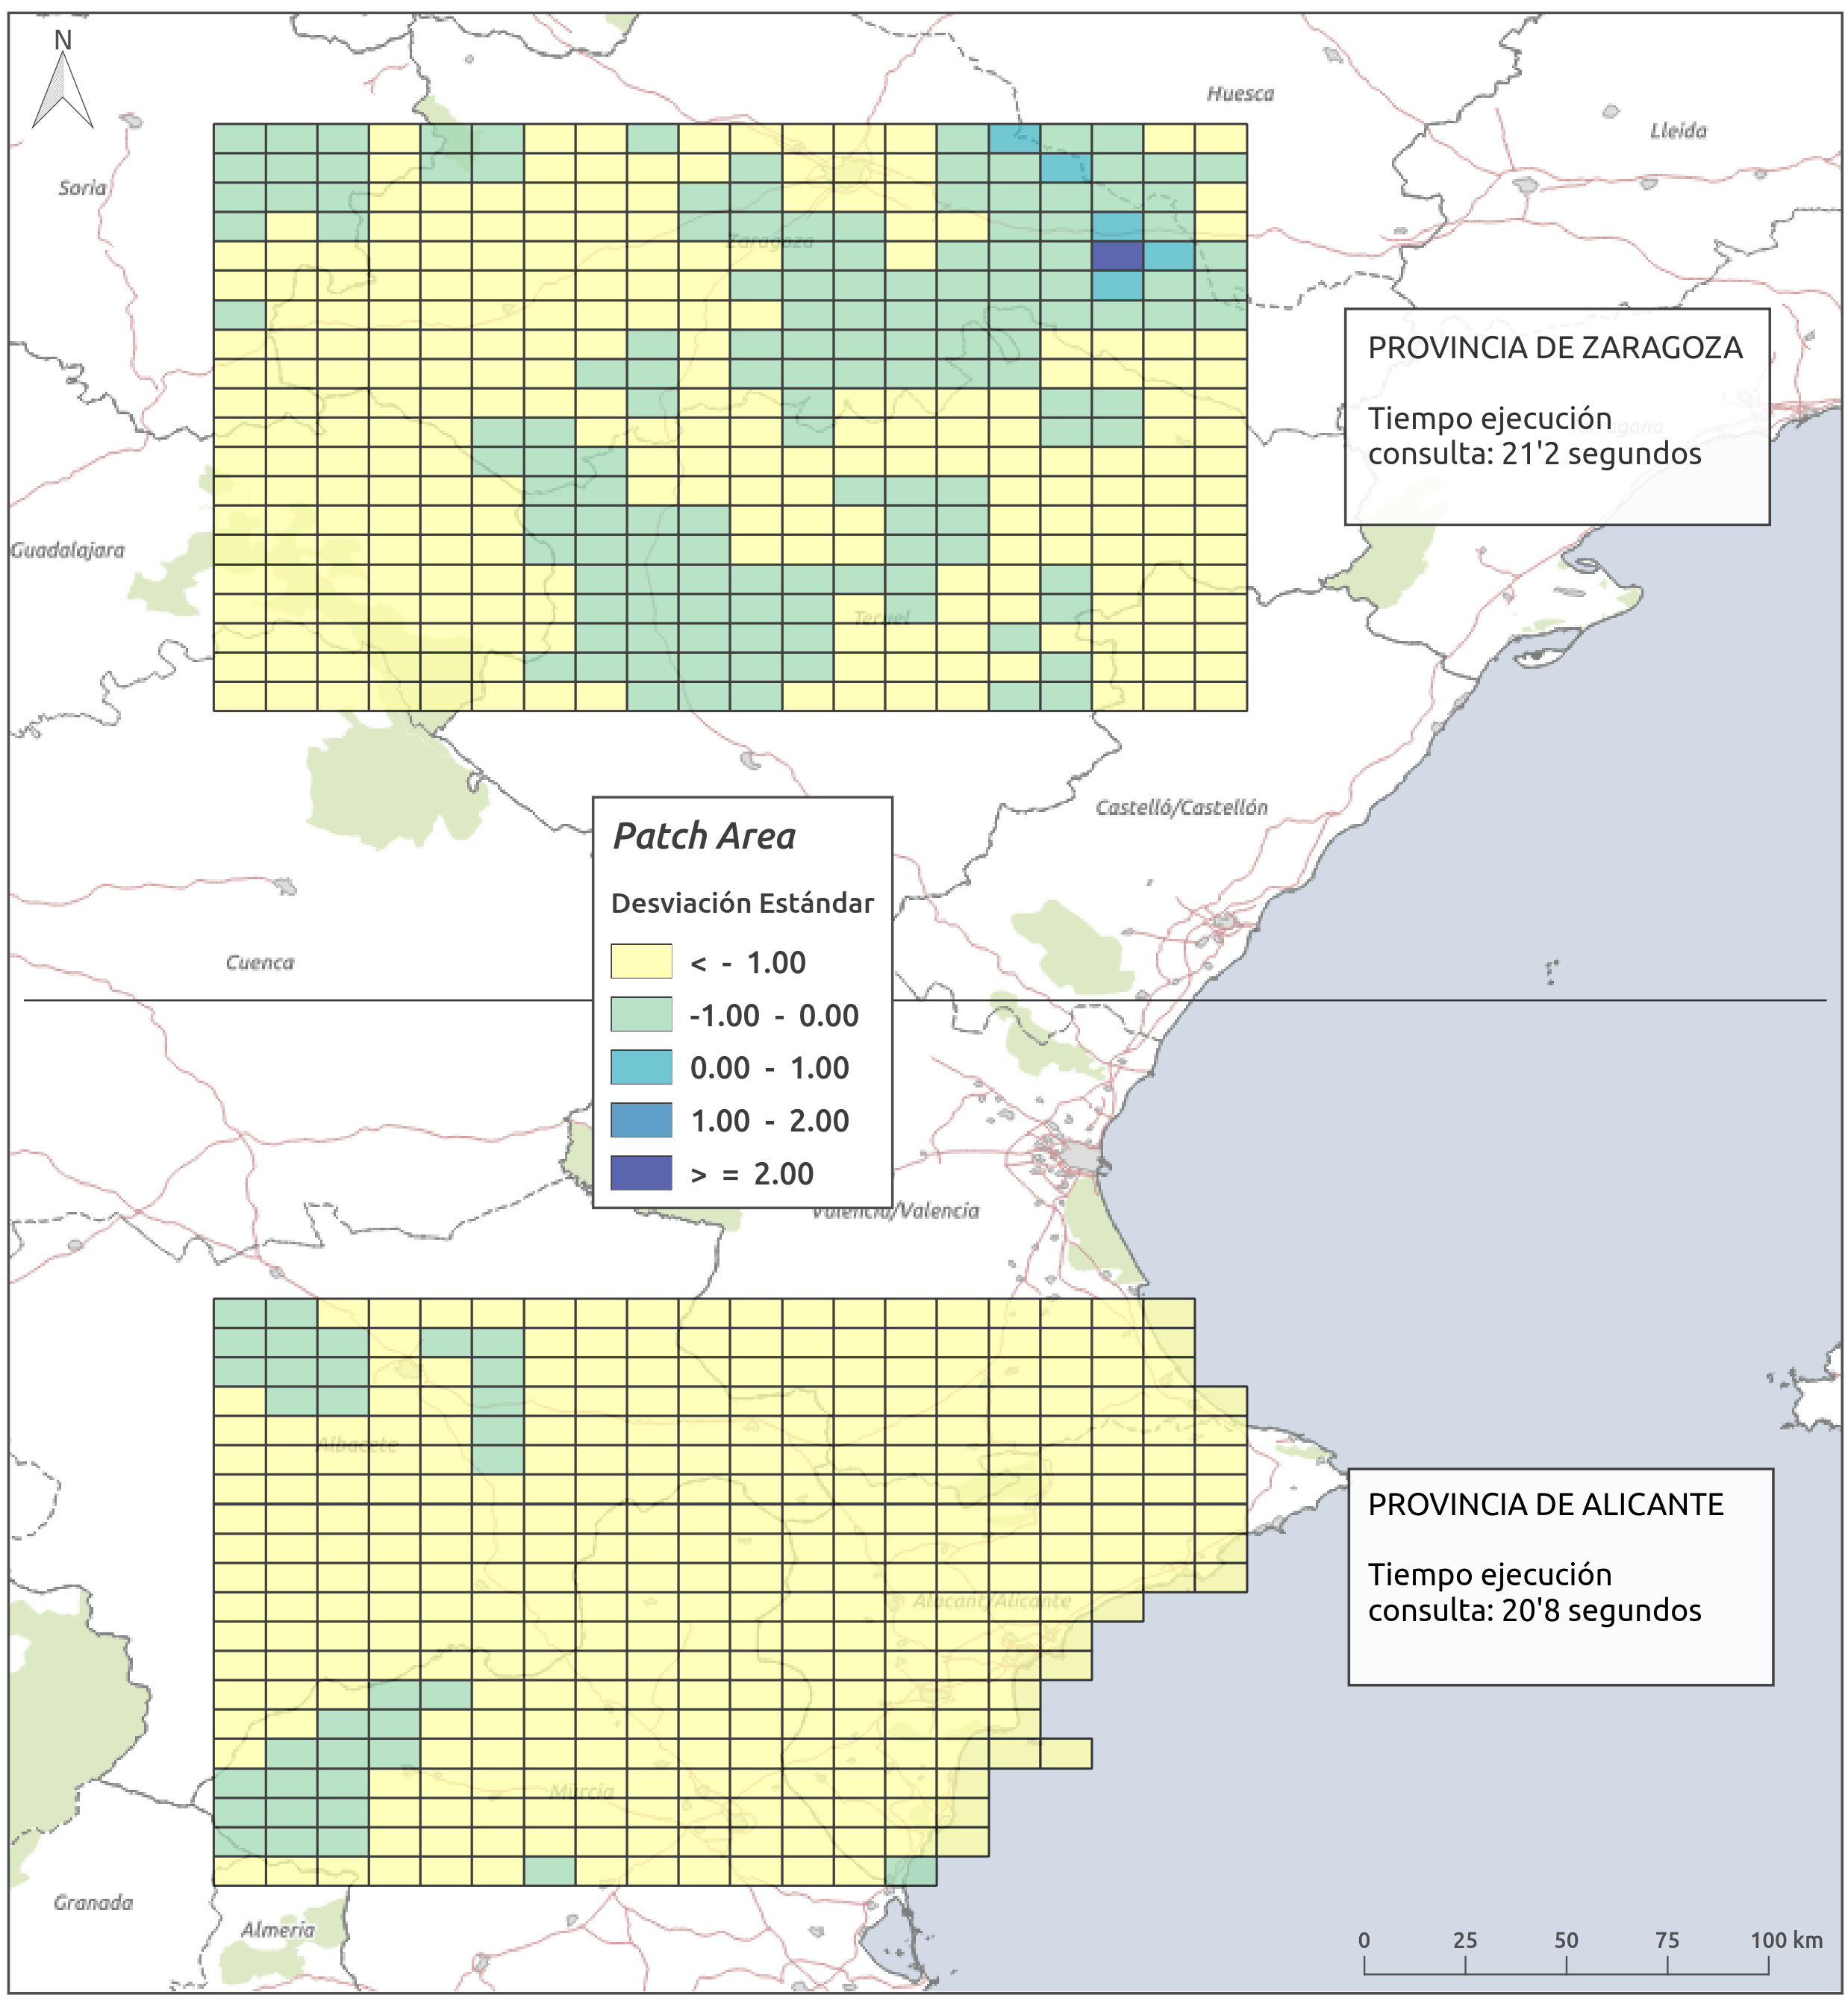
\includegraphics[width=\textwidth]{ResultadosyDiscusion/Figs/Results/p_25.png}
\caption{Calendario de actividad y contribuciones de este trabajo al proyecto \textit{pg\_landmetrics} (\textit{heatmap calendar}). \label{fig:p_25}}
\end{center}
\end{figure}

\begin{figure}
\begin{center}
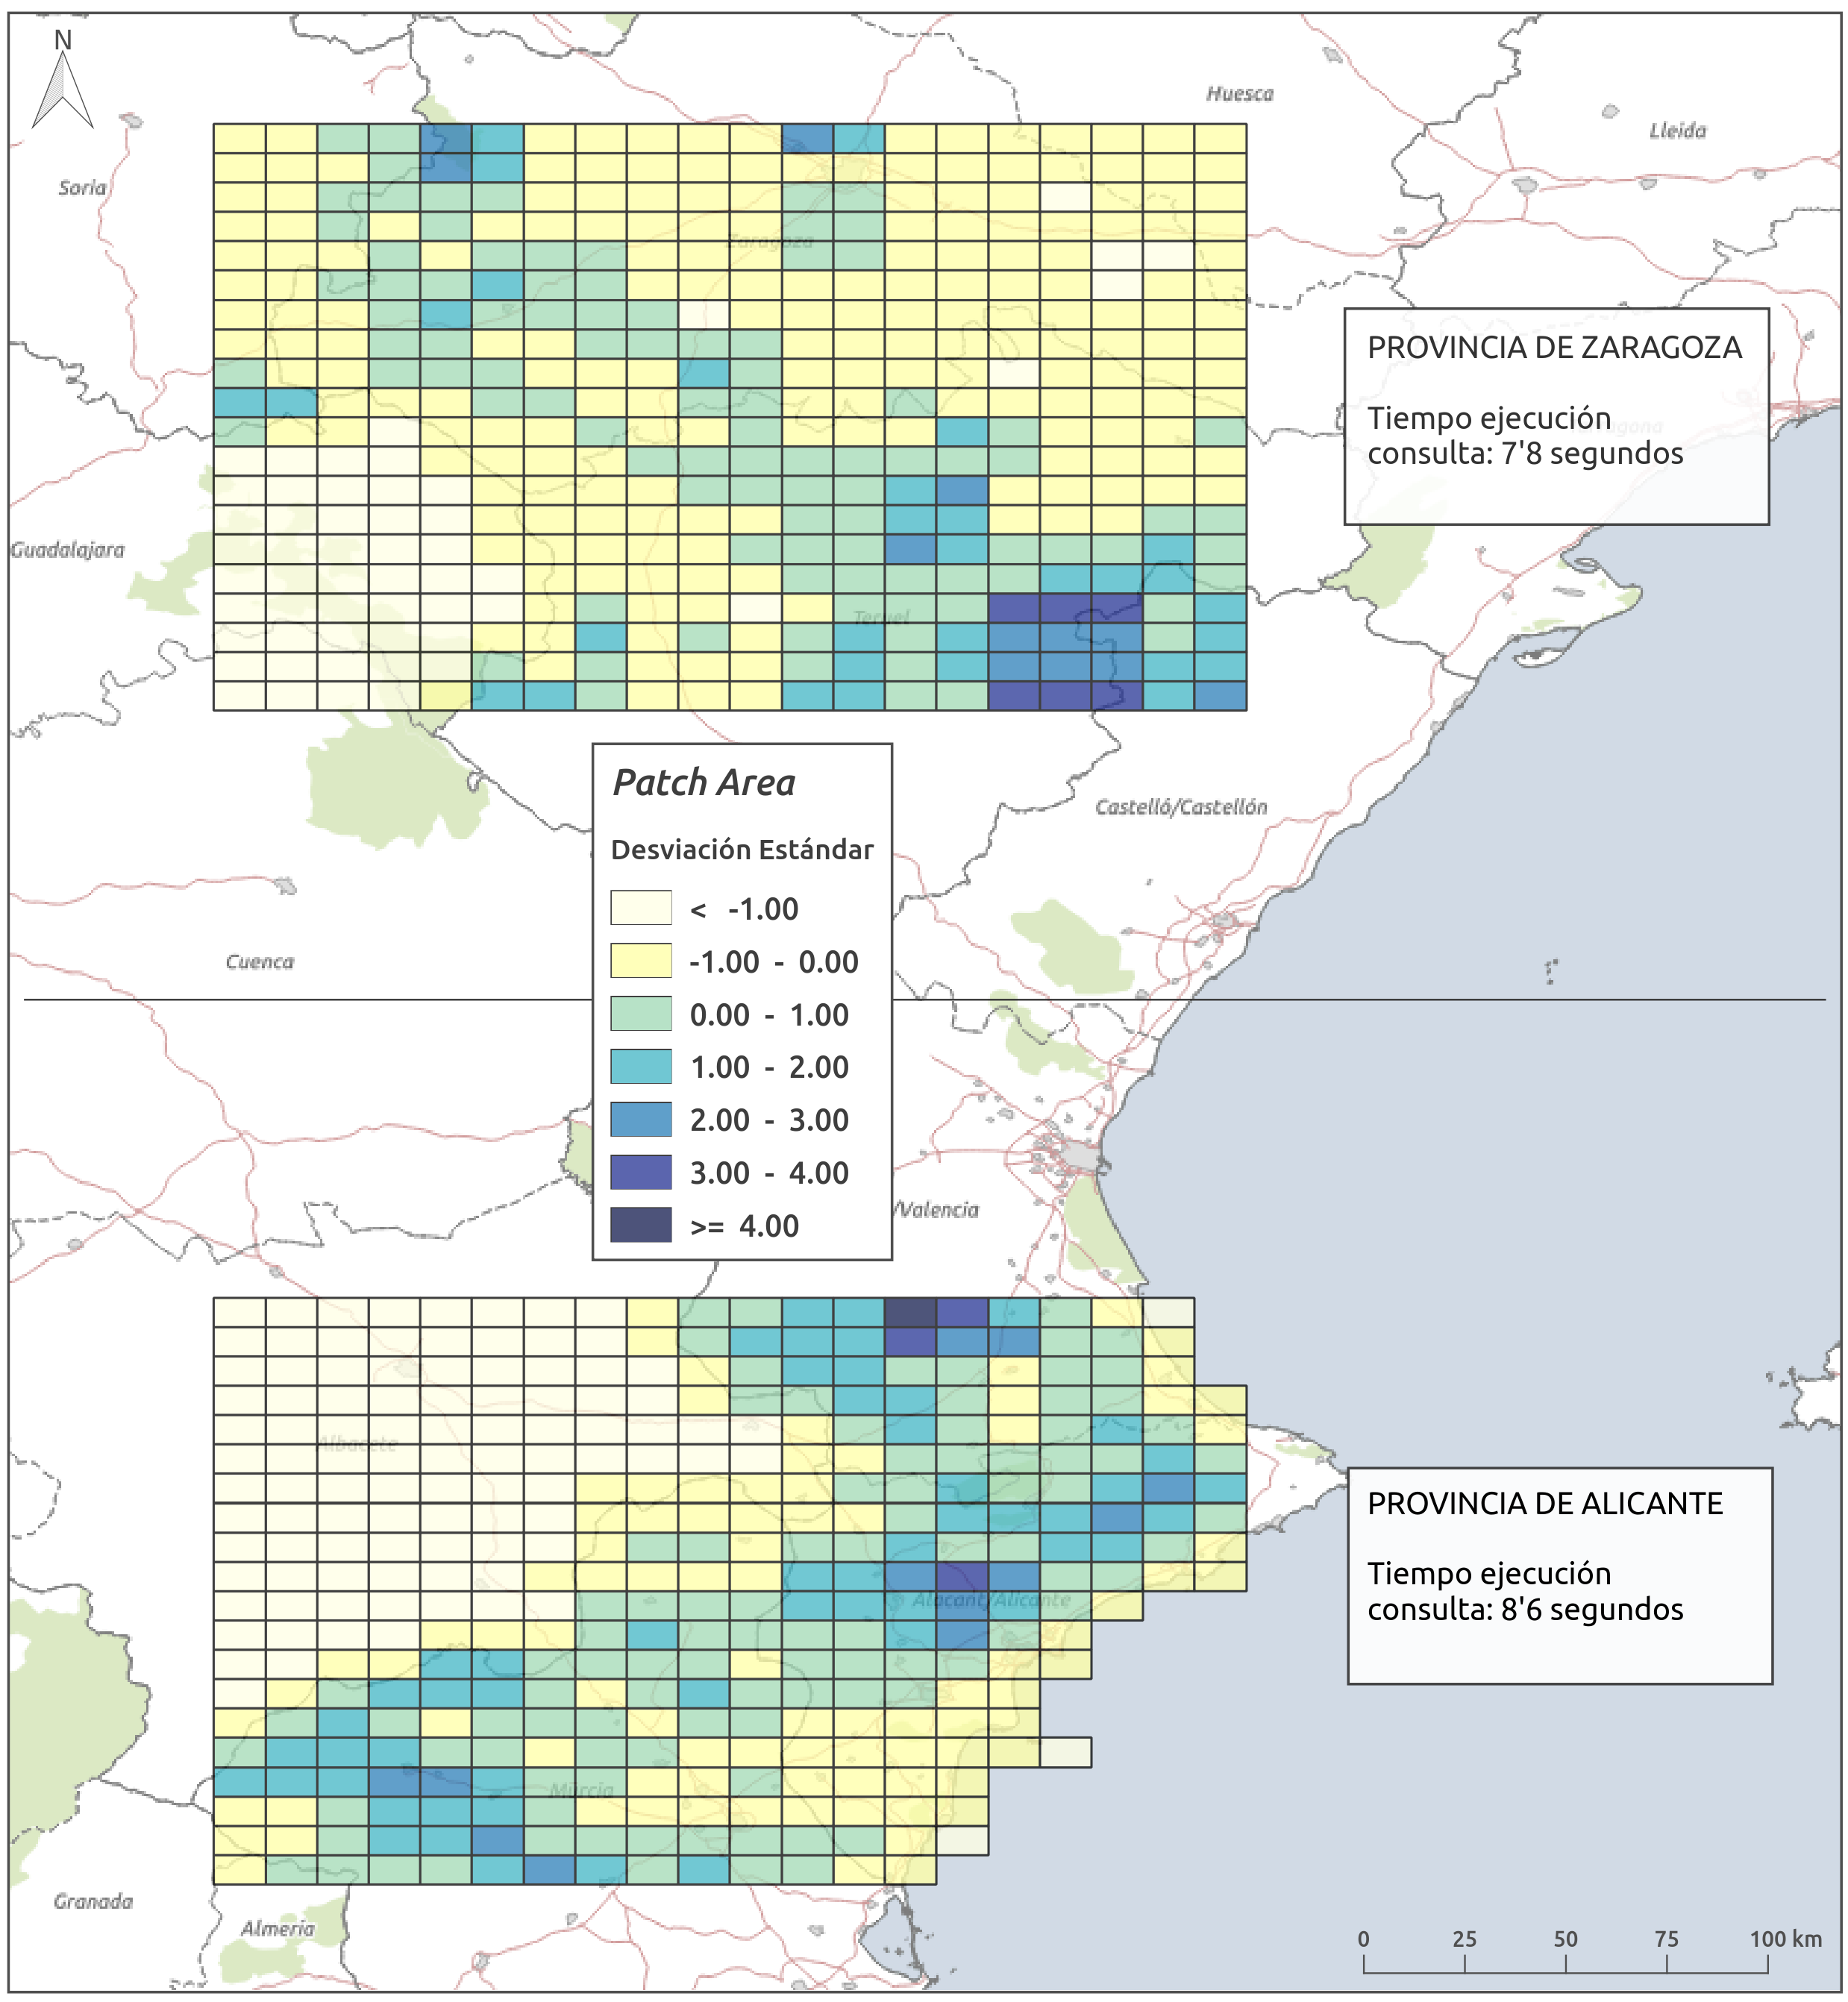
\includegraphics[width=\textwidth]{ResultadosyDiscusion/Figs/Results/c_25.png}
\caption{Calendario de actividad y contribuciones de este trabajo al proyecto \textit{pg\_landmetrics} (\textit{heatmap calendar}). \label{fig:c_25}}
\end{center}
\end{figure}

%!TEX root = ../thesis.tex
%*******************************************************************************
%****************************** Third Chapter **********************************
%*******************************************************************************
\chapter{Conclusiones y trabajo futuro}\label{chap:concl}

\begin{graybox}
\begin{itemize}
\item La extensión \pgland{} simplifica algunas complejas consultas SQL que son necesarias para calcular métricas del paisaje en una geodatabase.
\item El rendimiento de las consultas resulta prometedor, lo que permitirá crear servicios web de consulta directa sobre el SIOSE y bases de datos similares.   
\item El trabajo con \textit{dockers} facilita la reproducibilidad de la investigación y un despliegue escalable en Internet.
\item Los conocimientos adquiridos en el Máster sirven como introducción campos profesionales muy amplios.
\end{itemize}
\end{graybox}

Los objetivos planteados en el capítulo de \nameref{chap:intro} comprendian aspectos de trabajo colaborativo, cuestiones tecnológicas y había una gran preocupación por mejorar la \textit{usabilidad} de bases de datos voluminosas y complejas como la del SIOSE. En este sentido, el objetivo principal se ha conseguido al contribuir significativamente en el \textbf{desarrollo de una extensión de Postgres/PostGIS que facilita en gran medida el cálculo de métricas del paisaje}. 

La encapsulación del cálculo de métricas del paisaje en funciones de PostgreSQL/PostGIS facilita en gran medida la realización de estos cálculos a partir de bases de datos de ocupación del suelo como la del SIOSE. Esta facilidad se evidencia en la \textbf{reducción del número de líneas de SQL necesarias para el cálculo de las distintas métricas del paisaje}. Además, el desarrollo de nuevas métricas se ha podido sistematizar gracias a la gran extensibilidad de PostgreSQL/PostGIS. El uso de las más recientes tecnologías (\textit{Git y Dockers}) permite repartir el trabajo de desarrollo en equipos multidisciplinares, como lo es el del Laboratorio de Geomática de la Universidad de Alicante.

En este trabajo se ha obtenido un prototipo de una aplicación que, según los objetivos del Proyecto SIOSE-INNOVA, se pretende desarrollar en unos tres años. El desarrollo de una extensión \textit{en producción} llevará más tiempo, es un trabajo complejo que requiere de todo un equipo de expertos y meses de trabajo, es por ello que \textbf{el trabajo en equipo es esencial en este tipo de proyectos.}

\begin{figure}
\begin{center}
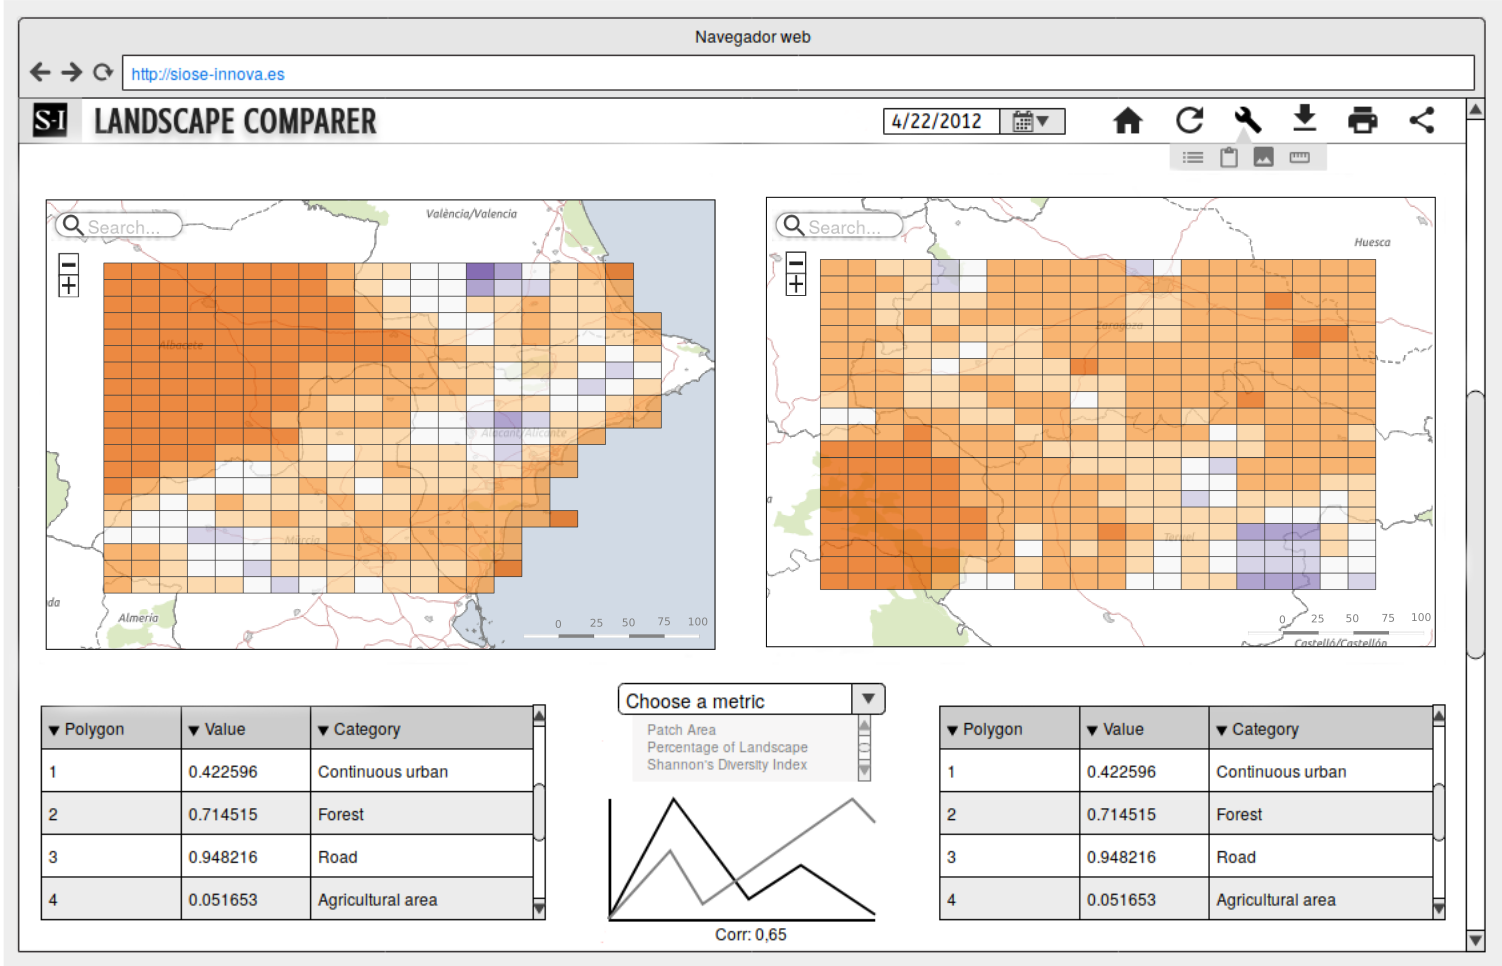
\includegraphics[width=\textwidth]{ConclusionyFuturo/Figs/visor-final.png}
\caption{Ejemplo de comparación de estructuras de paisaje a partir del SIOSE mediante el visor cartográfico . \label{fig:visor-final}}
\end{center}
\end{figure}

Los resultados obtenidos en el caso de uso descrito en las secciones \ref{sec:exp} y \ref{sec:caso_uso} han servido para poner a prueba la extensión y el resto de tecnologías en cuanto a su potencial de aplicación. Directamente sobre la geodatabase del SIOSE, se ha comprobado que es posible realizar centenares de consultas sobre métricas del paisaje en unos pocos segundos, y todo ello en un ordenador de sobremesa. Más aún, las nuevas tecnologías de contenerización utilizadas (\textit{Dockers}) permiten desplegar y distribuir toda la plataforma descrita en este trabajo en uno o varios servidores de Internet, por lo que cabe pensar que este tipo de servicios podrían ser ofrecidos a un gran número de usuarios del SIOSE.

Tras redactar este trabajo es posible valorar aún más los contenidos del ``Máster en Tecnologías de la Información Geográfica para la Ordenación del Territorio: SIG y Teledetección''. En las asignaturas de \textit{fundamentos teóricos sobre bases de datos, diseño e implementación de bases de datos, lenguajes de programación, software libre, análisis espacial básico, análisis visual de imágenes y desarrollo e implementación de la información geográfica en aplicaciones infográficas} se adquirieron conocimientos básicos para empezar a trabajar en un proyecto avanzado sobre geodatabases, como el propuesto en el marco del proyecto SIOSE-INNOVA.





% ********************************** Back Matter *******************************
% Backmatter should be commented out, if you are using appendices after References
%\backmatter

% ********************************** Bibliography ******************************
\begin{spacing}{0.9}

% To use the conventional natbib style referencing
% Bibliography style previews: http://nodonn.tipido.net/bibstyle.php
% Reference styles: http://sites.stat.psu.edu/~surajit/present/bib.htm


\bibliographystyle{apalike}
%\bibliographystyle{unsrt} % Use for unsorted references  
%\bibliographystyle{plainnat} % use this to have URLs listed in References
\cleardoublepage
\bibliography{Bibliografia/bibliografia} % Path to your References.bib file


% If you would like to use BibLaTeX for your references, pass `custombib' as
% an option in the document class. The location of 'reference.bib' should be
% specified in the preamble.tex file in the custombib section.
% Comment out the lines related to natbib above and uncomment the following line.

%\printbibliography[heading=bibintoc, title={References}]


\end{spacing}

% ********************************** Appendices ********************************

\begin{appendices} % Using appendices environment for more functunality

%!TEX root = ../thesis.tex
% ******************************* Thesis Appendix A ****************************
\chapter{Anexo}\label{Anexo}

\section*{Windows OS}

\subsection*{TeXLive package - full version}
\begin{enumerate}
\item	Download the TeXLive ISO (2.2GB) from\\
\href{https://www.tug.org/texlive/}{https://www.tug.org/texlive/}
\item	Download WinCDEmu (if you don't have a virtual drive) from \\
\href{http://wincdemu.sysprogs.org/download/}
{http://wincdemu.sysprogs.org/download/}
\item	To install Windows CD Emulator follow the instructions at\\
\href{http://wincdemu.sysprogs.org/tutorials/install/}
{http://wincdemu.sysprogs.org/tutorials/install/}
\item	Right click the iso and mount it using the WinCDEmu as shown in \\
\href{http://wincdemu.sysprogs.org/tutorials/mount/}{
http://wincdemu.sysprogs.org/tutorials/mount/}
\item	Open your virtual drive and run setup.pl
\end{enumerate}


\end{appendices}

% *************************************** Index ********************************
\printthesisindex % If index is present

\end{document}
